% By Ben-Kaniobi
% https://gist.github.com/Ben-Kaniobi


\documentclass[enabledeprecatedfontcommands]{scrartcl}

%\usepackage[ansinew]{inputenc}  % Schriftcodierung für Windows
\usepackage[utf8]{inputenc}
\usepackage[T1]{fontenc}        % Schriftkodierung
\usepackage{fancyhdr}

\usepackage[ngerman]{babel}     % Neue de. Rechtschr. (Worttrennung, äöüß etc.) als Parameter für babel
\usepackage{lmodern}            % Darstellung
\usepackage{wasysym}            % Spezielle Symbole
\usepackage{todonotes}          % ToDo-Notizen
\usepackage{perpage}
\usepackage{graphicx}
\usepackage{listings}
\usepackage{fancyhdr}
\usepackage{tabularx}
\usepackage{setspace} 
\usepackage[ngerman]{varioref}
\usepackage[ngerman]{babel}
\usepackage{ngerman}
% Bibliographie
\usepackage{bibgerm}
\usepackage{svg}
%\usepackage{calc}               % Erweiterte Berechnungen/Text messen
%\usepackage{amsmath}  % Math
%\usepackage[final]{pdfpages}   % PDF einbinden
\usepackage{siunitx}
\sisetup{locale=DE}
\usepackage[ % Hyperlinks (Muss das letzte geladene Paket sein)
unicode=false, % non-Latin Zeichen
pdftoolbar=true, % PDF-Viewer Toolbar
pdfmenubar=true, % PDF-Viewer Menü?
pdffitwindow=true, % Fenster an Seite anpassen beim Öffnen
pdfnewwindow=true, % Links in neuem Fenster
colorlinks=true, % false: Boxen-Links; true: Farben-Links
linkcolor=black, % Farbe von internen Links
citecolor=black, % Farbe von Links zu Bibliography
filecolor=magenta, % Farbe von Links zu Dateien
urlcolor=blue % Farbe von externen Links
]{hyperref}

%Layout for lstlistings
\lstloadlanguages{Java} % Java-Sprache laden, notwendig wegen option 'savemem'
\lstset{
  language=Java,
  numbers=left,
  numberstyle=\tiny,
  numbersep=5pt,
  literate=%
    {Ö}{{\"O}}1
    {Ä}{{\"A}}1
    {Ü}{{\"U}}1
    {ß}{{\ss}}1
    {ü}{{\"u}}1
    {ä}{{\"a}}1
    {ö}{{\"o}}1
    {°}{{$^\circ$}}1, 
  basicstyle=\fontfamily{pcr}\selectfont\scriptsize,
  showspaces=false,
  showtabs=false,
  showstringspaces=false,
  keywordstyle=\bfseries,
  tabsize=4,
  frameround=ffff,
  extendedchars=true,
  commentstyle=\itshape,
  postbreak=\space,
  breakindent=5pt,
  breaklines=true
}


 \pagestyle{fancy}
\setlength{\headheight}{70.55003pt}
\fancyhead{}
\fancyhead[LO,RE]{Software--Projekt 2\\ WiSe 2018/2019
	\\Testprotokoll}
\fancyhead[LE,RO]{Seite \thepage\\\slshape \leftmark\\\slshape \rightmark}

\MakePerPage{footnote}
% Subsection mit Normalem Text neben Titel
\newcommand{\subsectiont}[2]{\subsection[#1]{#1{\normalsize\normalfont #2}}}
% Autoref-Name von \subsection auf "Test"
\addto\extrasngerman{\def\subsectionautorefname{Test}}


%\newcommand{\hardwareinfo}{STM32 F4 Discovery Board mit RoboBoard}
%\newcommand{\hex}[1]{#1\textsubscript{hex}}%h}}%(16)}}

% Checkboxen
\newcommand{\platz}{\textcolor{white}{$\Box$}}
\newcommand{\leer}{$\Box$}
\newcommand{\ok}{$\CheckedBox$}
\newcommand{\nok}[1]{#1}%\mbox{\ooalign{\leer\cr\hidewidth \textcolor{red}{#1}\hidewidth\cr}}}

% Punktstyles global ändern
\renewcommand{\labelitemii}{$\circ$}
\renewcommand{\labelitemiii}{$\cdot$}
\setlength{\parindent}{0pt}

% Command um Space vor (Sub)Sections zu verkleinern, damit Fazit noch auf 1. Seite
%\newcommand{\cheat}{\vspace{-0.3mm}} % Damit Fazit noch auf gleicher Seite

\begin{document}
\thispagestyle{fancy}
\fancyhead[LO,RE]{ }
\fancyhead[LE,RO]{Universität Bremen\\FB 3 -- Informatik\\
	Prof. Dr. Rainer Koschke \\TutorIn: Marcel Steinbeck}
\fancyfoot[C]{}
% Start Titelseite
\vspace{3cm}

\begin{minipage}[H]{\textwidth}
	\begin{center}
		\bf
		\Large
		Software--Projekt 2 WiSe 2018/2019\\
		\smallskip
		\small
		VAK 03-BA-901.02\\
		\vspace{3cm}
	\end{center}
\end{minipage}
\begin{minipage}[H]{\textwidth}
	\begin{center}
		\vspace{1cm}
		\bf
		\Large Testprotokoll: GraphIt\\
		Black-Box-Test\\
		\vspace{1cm}
		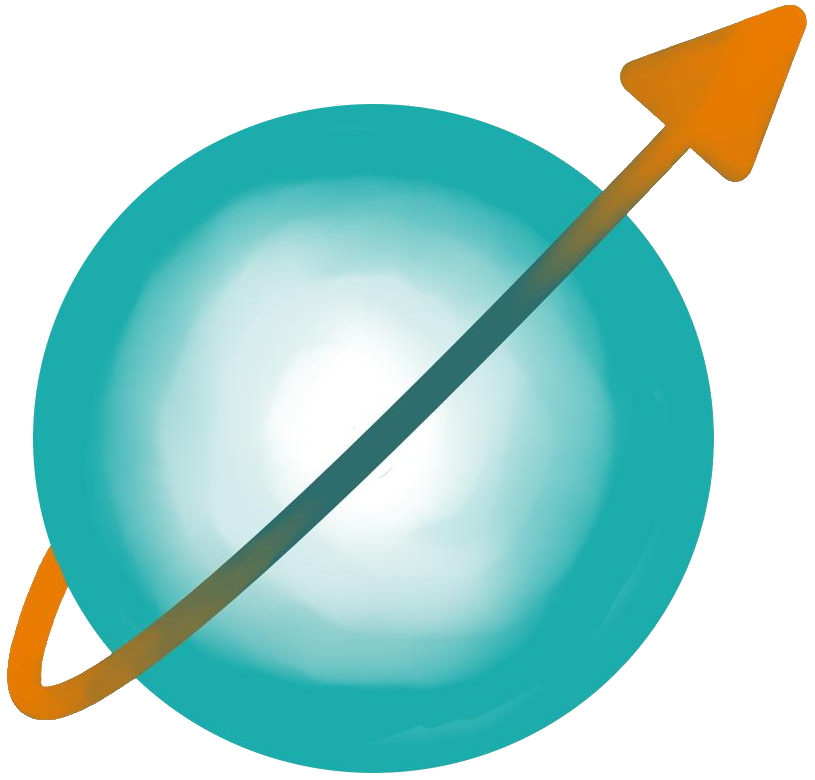
\includegraphics[width=2.5in]{logo_graphit.png}		
	\end{center}	
\end{minipage}
\vfill
\begin{minipage}[H]{\textwidth}
	\begin{center}
		\sf
		\begin{tabular}{lr}
			Anthony Mendil & antmen@tzi.de \\
			Bastian Rexhäuser & brexhaeu@tzi.de\\
			Clement Phung & clement1@tzi.de \\
			Jacky Philipp Mach & machja@tzi.de \\
			Jonah Jaeger & jjaeger@tzi.de \\
			Nina Unterberg & nin\_unt@tzi.de \\
		\end{tabular}
		\\ ~
		\vspace{2cm}
		\\
		\it Abgabe: 10. März 2019 --- Version 1.0\\ ~
	\end{center}
\end{minipage}


% Ende Titelseite	
	
\newpage
\textbf{\textcolor{red}{Anmerkungen!}}\\
Weil für manche Tests bestimmte Funktionalitäten funktionieren müssen, bauen die Tests aufeinander auf. Beispielsweise wird beim Testfall \texttt{Knoten hinzufügen} davon ausgegangen, dass nach dem vorherigen Testfall \texttt{Sphären hinzufügen} entsprechende Sphären existieren und somit nicht noch vorher erstellt werden müssen. \\
Ebenso wird beispielsweise beim Hinzufügen einer Sphäre nicht explizit erwähnt, dass in der Gui der Button zum Hinzufügen von Sphären betätigt wird. Sofern es nicht anders beschrieben ist, soll im folgenden also davon ausgegangen werden, dass bei den jeweiligen Aktionen des Testers die entsprechenden Buttons in der Kopfleiste der Gui betätigt werden. \\
Des weiteren wird im folgenden nicht jedes mal erwähnt, dass das Auswählen von einzelnen Elementen mithilfe eines Linksklick geschieht, beziehungsweise Umschalten (Shift) und Linksklicks für mehrere Elemente. \\
Bewegt werden Elemente durchs gedrückt Halten des Rechtsklicks. \\
Vor dem eigentlichen Testen der Anwendung sind im folgenden Bilder der Benutzeroberfläche zu sehen. Bei Testfällen, bei denen alle Tests negativ ausgefallen sind, sind Abbildungen (sofern vorhanden) nach den Tests zu finden und beziehen sich auf alle Testdurchläufe des entsprechenden Testfalls. Andernfalls werden bei jedem Testdurchlauf Abbildungen gezeigt (sofern vorhanden). \\
Auch hat sich im Verlauf bei der Erstellung des Testprotokolls die Standardfarben für Sphären und Symptomen geändert, was bei einigen Abbildungen zu erkennen ist.  \\

\newpage

\thispagestyle{fancy}
\fancyhead{}
\fancyhead[LO,RE]{Software--Projekt \\  2018/2019
	\\Testprotokoll}

\fancyhead[LE,RO]{Seite \thepage\\\slshape \leftmark\\~}
\fancyfoot{}
\renewcommand{\headrulewidth}{0.4pt}
\tableofcontents

\newpage


\fancyhead[LE,RO]{Seite \thepage\\\slshape \leftmark}
\section{Bilder der Benutzeroberfläche}
\emph{Autoren: Philipp Jacky Mach, Anthony Mendil}\\ 

Die Benutzeroberfläche im Ersteller-Modus:
\begin{center}
	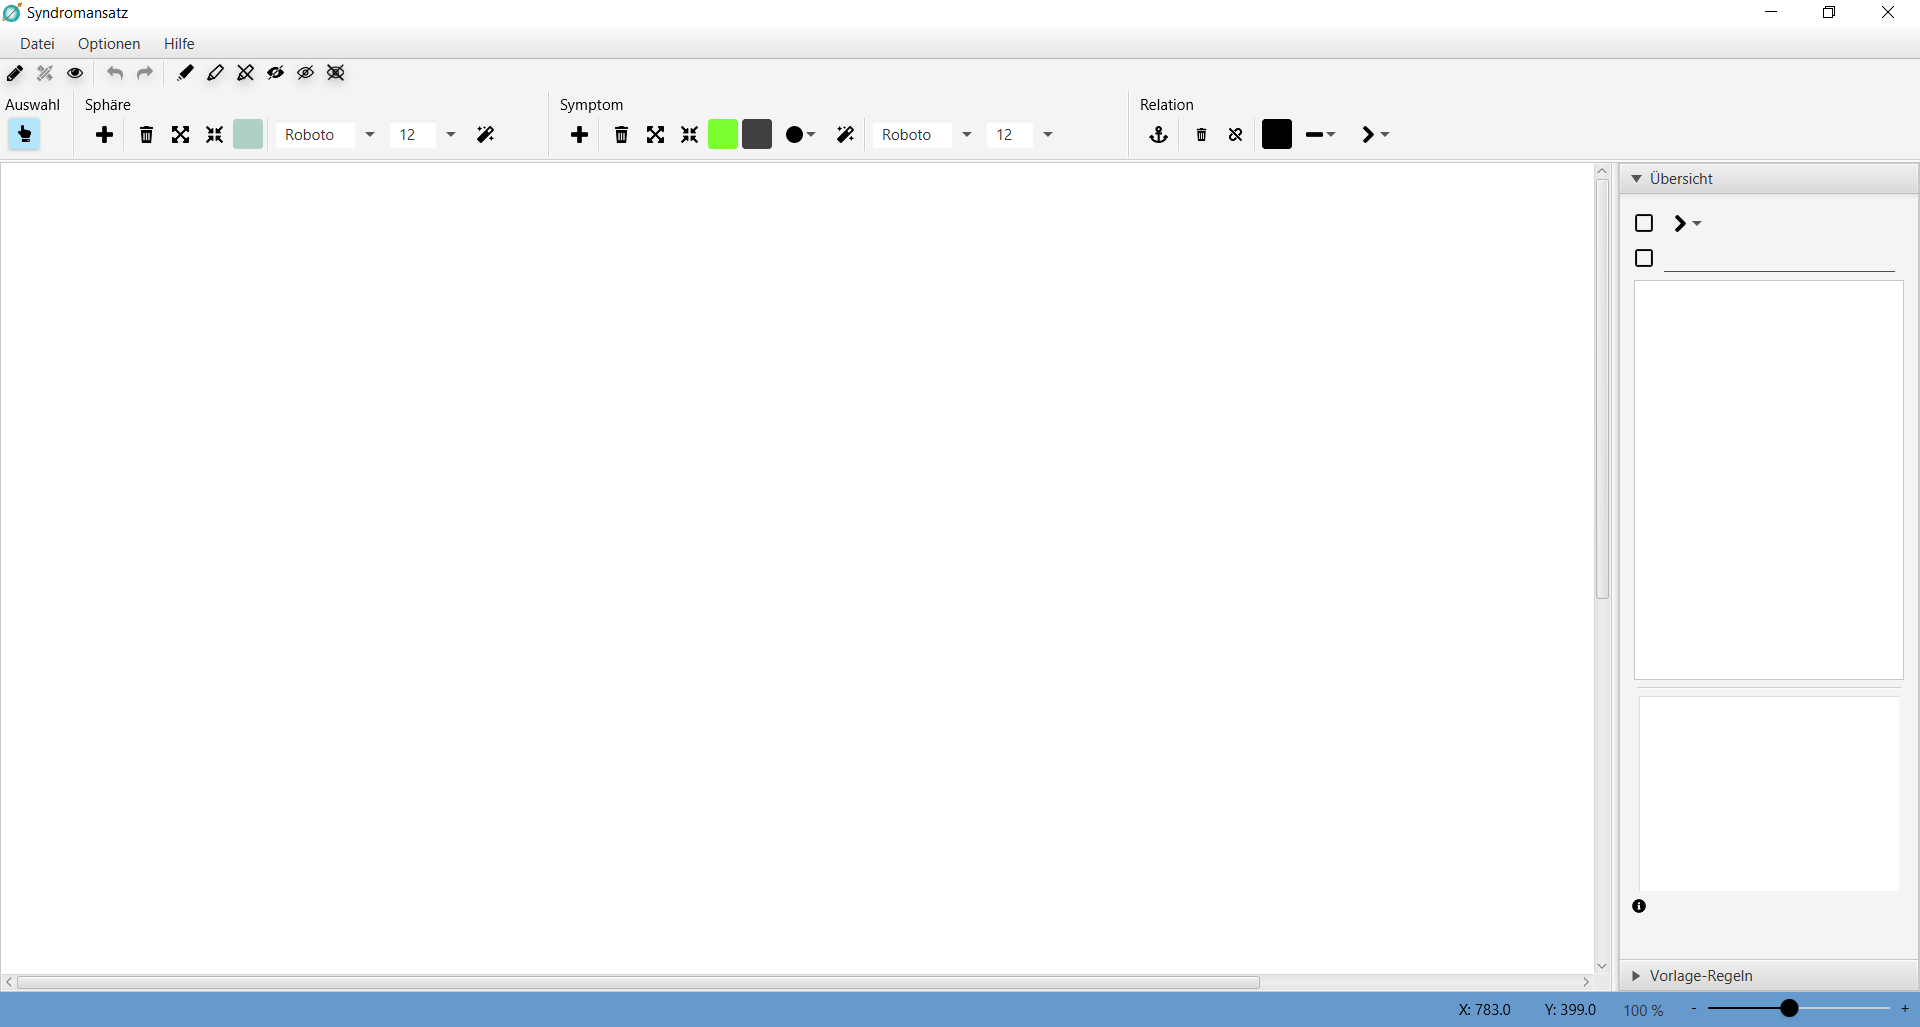
\includegraphics[height=9cm, angle = 90]{erstellerModus.png}
\end{center}
\newpage
Der einzige Unterschied zur Benutzeroberfläche im Bearbeiter-Modus ist der, dass es in der Seitenleiste zusätzlich zu den Vorlage-Regeln den Verlauf gibt,
wobei aber die Vorlage-Regeln nicht editierbar sind, sondern nur zum Lesen der Regeln dient:
\begin{center}
	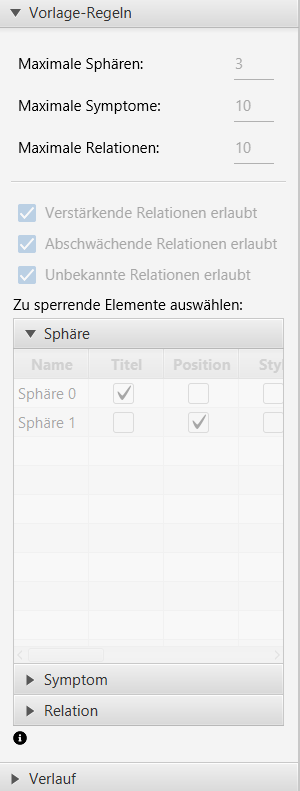
\includegraphics[height=10cm]{bearbeiterModus.PNG}
\end{center}
Was den Analyse-Modus von den anderen unterscheidet, ist die Kopfleiste und dass es keine Vorlage-Regeln gibt:
\begin{center}
	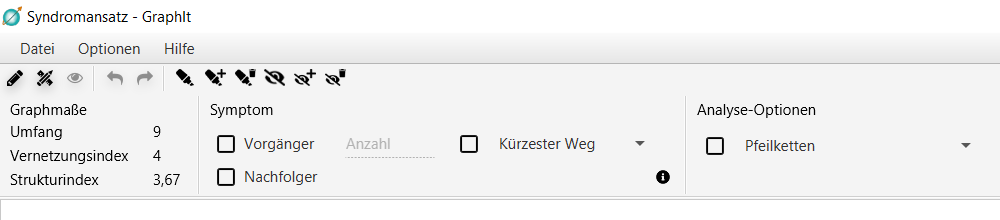
\includegraphics[height=3cm]{analyseModus.png}
\end{center}
\newpage
\hfill Test Nr.: \setlength{\fboxsep}{1pt}\fbox{1}\fbox{2}\fbox{3}
\section{Ersteller-Modus}
\emph{Autoren: Philipp Jacky Mach, Anthony Mendil, Clement Phung}\\ 
\subsectiont{Sphären hinzufügen an freien Stellen}{\dotfill\ok\ok\leer}
Der Ersteller erstellt zuerst zwei Sphären an verschiedenen Positionen. Eine links und dann eine rechts.  
\subsubsection{Notizen}
1.Test: Getestet von: Anthony Mendil. Datum: 21.02.2019 um 17:04 \\
Test negativ. \\
2.Test: Getestet von: Jacky Philipp Mach. Datum: 03.03.2019 um 19:10 \\
Test negativ.
\begin{center}
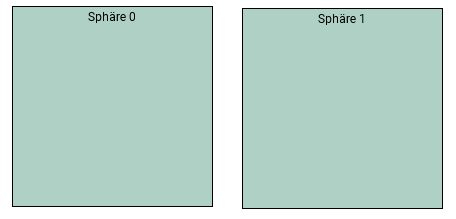
\includegraphics[height=5cm]{1_1.PNG}
\end{center}
\subsubsection{Fazit}
Die Software arbeitet wie erwartet.

\subsectiont{Sphäre hinzufügen, sodass es zu einer Überschneidung mit einer anderen kommen würde}{\dotfill\ok\ok\leer}
Der Ersteller versucht eine dritte Sphäre an einer Position hinzuzufügen, an der es zu einer Überschneidung mit einer der bereits erstellten Sphären kommen würde (nicht direkt auf der Sphäre). Hierbei ist zu erwarten, dass dies nicht erfolgreich ist und in der Fußleiste eine entsprechende Fehlermeldung angezeigt wird. 
\subsubsection{Notizen}
1.Test: Getestet von: Anthony Mendil. Datum: 21.02.2019 um 17:15 \\
Test negativ. \\
2.Test: Getestet von: Jacky Philipp Mach. Datum: 03.03.2019 um 19:12 \\
Test negativ.
\subsubsection{Fazit}
Die Software arbeitet wie erwartet. Die Abbildung ist identisch zur vorherigen.

\subsectiont{Knoten hinzufügen an freien Stellen in Sphären}{\dotfill\ok\ok\leer}
Es werden den zwei existierenden Sphären jeweils zwei Symptome an verschiedenen Positionen hinzugefügt. Erst in die linke Sphäre oben mittig und unten mittig und dann in die rechte Sphäre oben mittig und unten mittig.  
\subsubsection{Notizen}
1.Test: Getestet von: Anthony Mendil. Datum: 21.02.2019 um 17:20 \\
Test negativ.\\
2.Test: Getestet von: Jacky Philipp Mach. Datum: 03.03.2019 um 19:14 \\
Test negativ.
\begin{center}
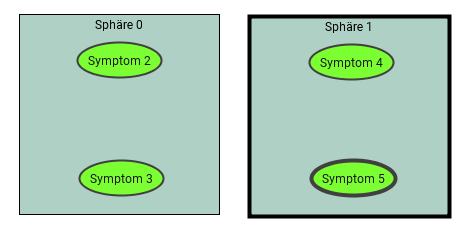
\includegraphics[height=5cm]{1_3.PNG}
\end{center}
\subsubsection{Fazit}
Die Software arbeitet wie erwartet.

\subsectiont{Knoten hinzufügen an belegter Stelle}{\dotfill\ok\ok\leer}
Der Ersteller versucht an einer Stelle innerhalb einer Sphäre ein Symptom hinzuzufügen, an der bereits ein anderes Symptom ist. Hierbei ist analog zu Sphären zu erwarten, dass dies nicht erfolgreich ist und in der unteren Leiste eine entsprechende Meldung angezeigt wird.
\subsubsection{Notizen}
1.Test: Getestet von: Anthony Mendil. Datum: 21.02.2019 um 17:30 \\
Test negativ.\\
2.Test: Getestet von: Jacky Philipp Mach. Datum: 03.03.2019 um 19:17 \\
Test negativ.
\subsubsection{Fazit}
Die Software arbeitet wie erwartet. Die Abbildung ist identisch zur vorherigen.

\subsectiont{Knoten hinzufügen außerhalb einer Sphäre}{\dotfill\ok\ok\leer}
Der Ersteller versucht an einer Stelle außerhalb einer Sphäre ein Symptom hinzuzufügen. Zu erwarten ist, dass dies nicht erlaubt wird. Durch eine Fehlermeldung in der Fußleiste sollte dies angezeigt werden. 
\subsubsection{Notizen}
1.Test: Getestet von: Anthony Mendil. Datum: 21.02.2019 um 17:39 \\
Test negativ.\\
2.Test: Getestet von: Jacky Philipp Mach. Datum: 03.03.2019 um 19:17 \\
Test negativ.
\subsubsection{Fazit}
Die Software arbeitet wie erwartet. Die Abbildung ist identisch zur vorherigen.

\subsectiont{Verstärkende Relation zwischen zwei Symptome der selben Sphäre}{\dotfill\ok\ok\leer}
Der Ersteller zieht eine verstärkende Relationen von \texttt{Symptom 2} nach \texttt{Symptom 3}. 
\subsubsection{Notizen}
1.Test: Getestet von: Anthony Mendil. Datum: 21.02.2019 um 17:39 \\
Test negativ.\\
2.Test: Getestet von: Jacky Philipp Mach. Datum: 03.03.2019 um 19:18 \\
Test negativ.
\begin{center}
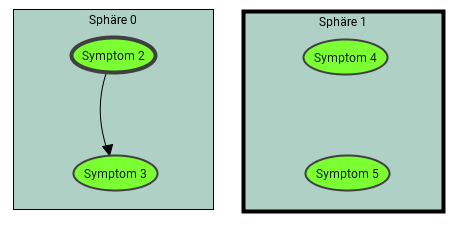
\includegraphics[height=5cm]{1_6.PNG}
\end{center}
\subsubsection{Fazit}
Die Software arbeitet wie erwartet.

\subsectiont{Rückgängig machen (Undo)}{\dotfill\ok\ok\leer}
Der Ersteller betätigt den Button zum Rückgängigmachen der letzten Aktion.
\subsubsection{Notizen}
1.Test: Getestet von: Anthony Mendil. Datum: 21.02.2019 um 17:45 \\
Test negativ.\\
2.Test: Getestet von: Jacky Philipp Mach. Datum: 03.03.2019 um 19:19 \\
Test negativ.
\begin{center}
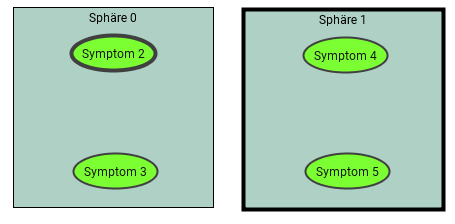
\includegraphics[height=5cm]{1_7neu.PNG}
\end{center}
\subsubsection{Fazit}
Die Software arbeitet wie erwartet.

\subsectiont{Wiederherstellen (Redo)}{\dotfill\ok\ok\leer}
Der Ersteller betätigt den Button zum Wiederherstellen der zuletzt rückgängig gemachten Aktion. 
\subsubsection{Notizen}
1.Test: Getestet von: Anthony Mendil. Datum: 21.02.2019 um 17:53 \\
Test negativ.\\
2.Test: Getestet von: Jacky Philipp Mach. Datum: 03.03.2019 um 19:20 \\
Test negativ.
\begin{center}
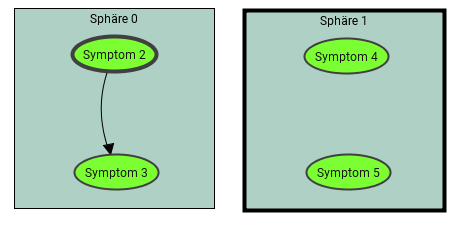
\includegraphics[height=5cm]{1_8neu.PNG}
\end{center}
\subsubsection{Fazit}
Die Software arbeitet wie erwartet.

\subsectiont{Relation zwischen zwei Symptomen, zwischen denen bereits eine Relation existiert}{\dotfill\ok\ok\leer}
Der Ersteller versucht jeweils eine verstärkende, eine unbekannte und eine abschwächende Relation.
\subsubsection{Notizen}
1.Test: Getestet von: Anthony Mendil. Datum: 21.02.2019 um 18:12 \\
Test negativ.\\
2.Test: Getestet von: Jacky Philipp Mach. Datum: 03.03.2019 um 19:25 \\
Test negativ.
\subsubsection{Fazit}
Die Software arbeitet wie erwartet. Die Abbildung ist identisch zur vorherigen.

\subsectiont{Abschwächende Relation zwischen zwei Symptomen unterschiedlicher Sphären}{\dotfill\ok\ok\leer}
Der Ersteller zieht eine abschwächende Relationen von \texttt{Symptom 2} nach \texttt{Symptom 5}. 
\subsubsection{Notizen}
1.Test: Getestet von: Anthony Mendil. Datum: 21.02.2019 um 17:39 \\
Test negativ.\\
2.Test: Getestet von: Jacky Philipp Mach. Datum: 03.03.2019 um 19:27 \\
Test negativ.
\begin{center}
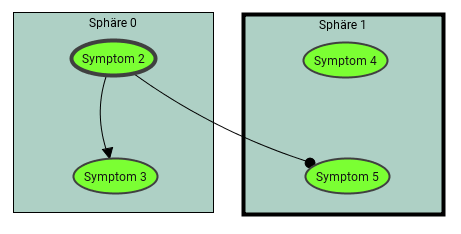
\includegraphics[height=5cm]{1_10.PNG}
\end{center}
\subsubsection{Fazit}
Die Software arbeitet wie erwartet.

\subsectiont{Unbekannte Relation zwischen zwei Symptomen\\ unterschiedlicher Sphären}{\dotfill\ok\ok\leer}
Der Ersteller zieht eine unbekannte Relationen von \texttt{Symptom 4} nach \texttt{Symptom 2}. 
\subsubsection{Notizen}
1.Test: Getestet von: Anthony Mendil. Datum: 21.02.2019 um 18:01 \\
Test negativ.\\
2.Test: Getestet von: Jacky Philipp Mach. Datum: 03.03.2019 um 19:29 \\
Test negativ.
\begin{center}
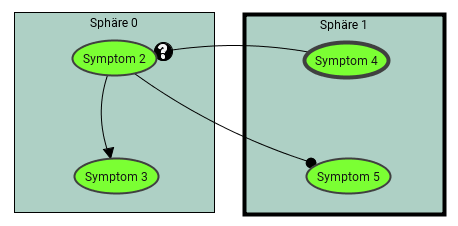
\includegraphics[height=5cm]{1_11.PNG}
\end{center}
\subsubsection{Fazit}
Die Software arbeitet wie erwartet.

\subsectiont{Einstellen der Vorlage-Regeln}{\dotfill\ok\ok\leer}
Der Ersteller öffnet in der rechten Seitenleiste die Vorlage Regeln. Er stellt ein, dass es nur maximal drei Sphären, zehn Symptome und zehn Relationen geben darf, sowie dass unbekannte und abschwächende Relationen nicht erlaubt sind. \\
Anschließend stellt er ein, dass der Titel sowie der Style von \texttt{Sphäre 0} nicht verändert werden darf und die Position von \texttt{Sphäre 1} nicht verändert werden darf. Ebenso dürfen \texttt{Sphäre 1} keine Symptome hinzugefügt werden und keine Symptome von ihr gelöscht werden. Trotzdem stellt der Ersteller
ein, das maximal 4 Symptome in \texttt{Sphäre 0} und maximal 3 Symptome in \texttt{Sphäre 1} erlaubt sind. \\
Bezüglich der Symptome wird eingestellt, dass der Titel von \texttt{Symptom 5}, die Position von \texttt{Symptom 3} und der Style von {Symptom 2} nicht verändert werden dürfen. \\
Abschließend stellt er noch ein, dass die Position der Relation von \texttt{Symptom 2} nach \texttt{Symptom 5}, der Style der Relation von \texttt{Symptom 4} nach \texttt{Symptom 2} und die Relationsart der Relation von \texttt{Symptom 2} nach \texttt{Symptom 3} nicht verändert werden dürfen. 
\subsubsection{Notizen}
1.Test: Getestet von: Anthony Mendil. Datum: 21.02.2019 um 18:01 \\
Test negativ. \\
2.Test: Getestet von: Jacky Philipp Mach. Datum: 03.03.2019 um 19:34 \\
Test negativ.
\begin{center}
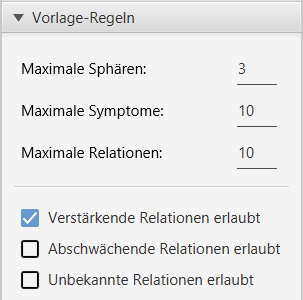
\includegraphics[height=5cm]{template4.png}
\end{center}
\begin{center}
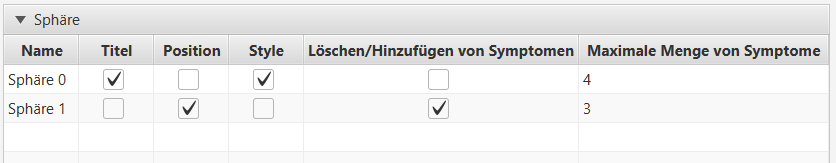
\includegraphics[height=3cm]{template1.PNG}
\end{center}
\begin{center}
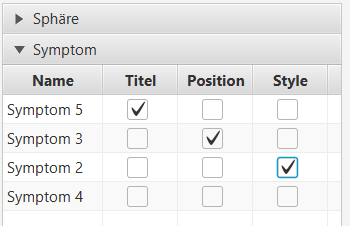
\includegraphics[height=5cm]{template2.PNG}
\end{center}
\begin{center}
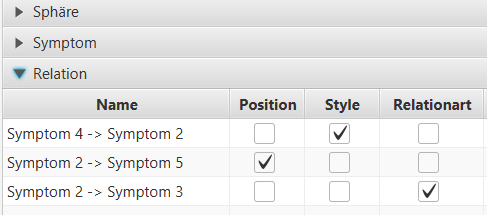
\includegraphics[height=5cm]{template3.png}
\end{center}
Da der Erzeuger gegen seine eigene Regeln verstoßen kann, müssen entsprechende Funktionalitäten im Bearbeiter-Modus getestet werden.
\subsubsection{Fazit}
Die Software arbeitet wie erwartet.

\subsectiont{Schließen des Programms ohne den Graphen zu speichern}{\dotfill\ok\ok\leer}
Der Ersteller schließt das Programm ohne vorher seinen Graphen zu speichern. Anschließend startet er das Programm erneut. Hierbei ist zu erwarten, dass der Graph identisch zu dem vor dem Schließen des Programms ist. 
\subsubsection{Notizen}
1.Test: Getestet von: Anthony Mendil. Datum: 21.02.2019 um 18:42 \\
Test negativ.\\
2.Test: Getestet von: Jacky Philipp Mach. Datum: 03.03.2019 um 14:38 \\
Test negativ.
\subsubsection{Fazit}
Die Software arbeitet wie erwartet. 

\subsectiont{Verstoß gegen die eigenen Vorlage-Regeln}{\dotfill\ok\ok\leer}
Der Ersteller versucht \texttt{Sphäre 1} zu bewegen. Obwohl das Bewegen dieser Sphäre in den Regeln verboten wird, sollte diese Aktion erfolgreich sein, weil der Ersteller gegen seine eigenen Regeln verstoßen darf. Analog zu diesem Testfall sollte der Tester versuchen auch gegen die anderen in den Vorlage-Regeln festgelegten Einschränkungen zu verstoßen. 
\subsubsection{Notizen}
1.Test: Getestet von: Anthony Mendil. Datum: 21.02.2019 um 18:52 \\
Test negativ. \\
2.Test: Getestet von: Jacky Philipp Mach. Datum: 03.03.2019 um 19:43 \\
Test negativ.
\begin{center}
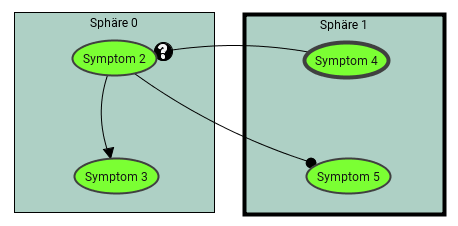
\includegraphics[height=5cm]{1_11.PNG}
\end{center}
\subsubsection{Fazit}
Die Software arbeitet wie erwartet.

\subsectiont{Entfernen einer Relation im Ersteller-Modus bei der in den Vorlage-Regeln das Verändern des Styles verboten wurde}{\dotfill\XBox\ok\leer}
Der Ersteller versucht die Relation von \texttt{Symptom 4} nach \texttt{Symptom 2} zu entfernen. Obwohl dies aufgrund der Vorlage-Regeln verboten wird, ist zu erwarten, dass die Relation entfernt wird, weil die Regeln nicht im Ersteller-Modus gelten sollen.
\subsubsection{Notizen}
1.Test: Getestet von: Anthony Mendil. Datum: 22.02.2019 um 13:56 \\
Test positiv, weil das Entfernen der Relation nicht erfolgreich war. Die Abbildung ist identisch zur vorherigen. \\ 
2.Test: Getestet von: Jacky Philipp Mach. Datum: 03.03.2019 um 19:43 \\
Test negativ. 
\newpage
Vor dem Entfernen der Relation:
\begin{center}
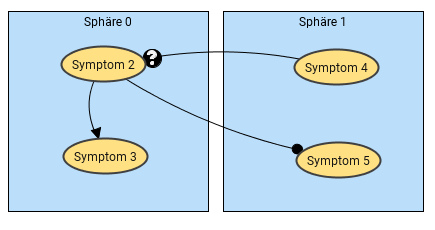
\includegraphics[height=5cm]{1_15vorher.png}
\end{center}
Nach dem Entfernen der Relation:
\begin{center}
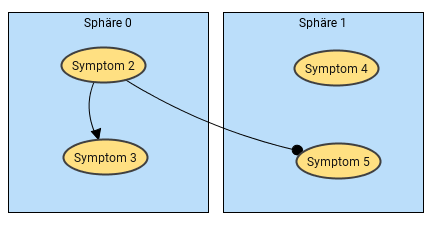
\includegraphics[height=5cm]{1_15nachher.png}
\end{center}

\subsubsection{Fazit} 
Die Abfrage des jetzigen Modus entsprach nicht dem geplanten. Nachdem der Boolesche Wert negiert worden ist, funktioniert dies nun wie erwartet.

\subsectiont{Speichern der Datei in den eigenen Dateien}{\dotfill\ok\ok\leer}
Der Ersteller speichert über \texttt{Datei} und \texttt{Speichern unter} die soeben erstellte Vorlage inklusive der Regeln. 
\subsubsection{Notizen}
1.Test: Getestet von: Anthony Mendil. Datum: 21.02.2019 um 19:00 \\
Test negativ.\\
2.Test: Getestet von: Jacky Philipp Mach. Datum: 03.03.2019 um 19:45 \\
Test negativ.
\subsubsection{Fazit}
Die Software arbeitet wie erwartet. In dem Verzeichnis das zum Speichern ausgewählt wurde ist die entsprechende Datei zu finden. 

\newpage

\section{Bearbeiter-Modus}
\emph{Autoren: Philipp Jacky Mach, Anthony Mendil, Clement Phung}\\ \\
Im Ersteller-Modus getestete Funktionalitäten, die auch im Bearbeiter-Modus zur Verfügung stehen, werden im Bearbeiter-Modus nicht nochmal explizit getestet. 

\subsectiont{Rückgängig machen einer Aktion die im Ersteller Modus durchgeführt wurde und in den Vorlage-Regeln verboten wurde}{\dotfill\XBox\ok\leer}
Hierfür wird vorerst im Ersteller-Modus eine Sphäre erstellt und in den Vorlage Regeln festgelegt, dass diese nicht bewegt werden kann (analog zu Testfall 1.10). Anschließend wird die Sphäre im Ersteller-Modus bewegt und direkt in den Bearbeiter-Modus gewechselt, wo der Button zum Rückgängigmachen der letzten Aktion betätigt wird. Hierbei ist zu erwarten, dass das Bewegen der Sphäre nicht rückgängig gemacht wird, weil das Bewegen dieser Sphäre in den Vorlage-Regeln verboten wurde. 
\subsubsection{Notizen}
1.Test: Getestet von: Anthony Mendil. Datum: 22.02.2019 um 11:39 \\
Test positiv, weil die Sphäre beim Betätigen des Buttons zum Rückgängigmachen bewegt wurde. \\
Vorher: 
\begin{center}
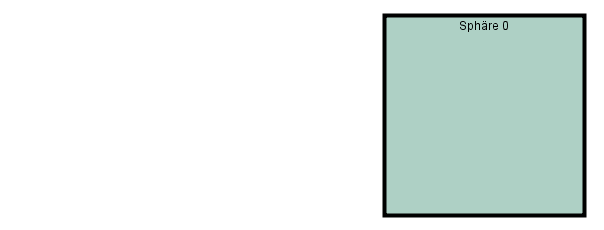
\includegraphics[height=5cm]{2_1vorher.PNG}
\end{center}
Nachher: 
\begin{center}
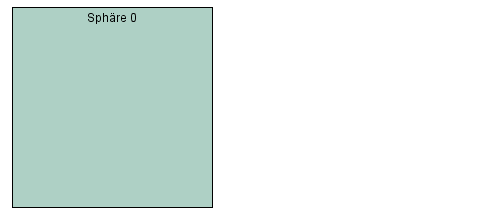
\includegraphics[height=5cm]{2_1nachher.PNG}
\end{center}
2.Test: Getestet von: Jacky Philipp Mach. Datum: 03.03.2019 um 19:47 \\
Test negativ. \\
Vorher: 
\begin{center}
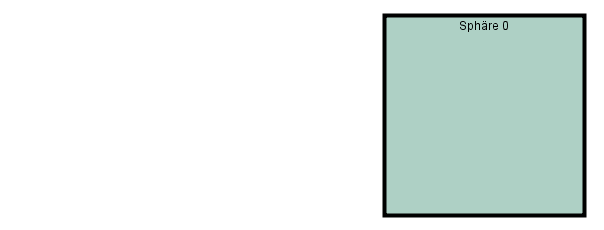
\includegraphics[height=5cm]{2_1vorher.PNG}
\end{center}
Nachher: 
\begin{center}
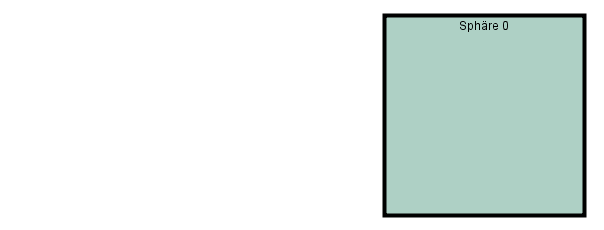
\includegraphics[height=5cm]{2_1vorher.PNG}
\end{center}
\subsubsection{Fazit}
Nach dem ersten Test wurde geändert, dass nach jeden Wechsel des Modus die \texttt{Action History} geleert wird.
Nach dem zweiten Test arbeitet die Software wie erwartet. 

\subsectiont{Datei Öffnen}{\dotfill\ok\ok\leer}
Der Ersteller drückt auf \texttt{Datei} und \texttt{Datei öffnen} und wählt im entsprechendem Verzeichnis die im Ersteller-Modus gespeicherte Datei aus. Zu erwarten ist, dass der Graph identisch zum im Ersteller-Modus erstellten ist. 
\subsubsection{Notizen}
1.Test: Getestet von: Anthony Mendil. Datum: 22.02.2019 um 10:32 \\
Test negativ.\\
2.Test: Getestet von: Jacky Philipp Mach. Datum: 03.03.2019 um 19:49 \\
Test negativ.
\subsubsection{Fazit}
Die Software arbeitet wie erwartet.

\subsectiont{Keinen Verlauf im Ersteller-Modus erstellen}{\dotfill\ok\ok\leer}
Im Ersteller-Modus soll der Verlauf bei der Erstellung des Graphen nicht aufgezeichnet werden. Deshalb ist im Bearbeiter-Modus, sofern man einen soeben erstellten Graphen geladen hat, zu erwarten, dass in der Seitenleiste der Verlauf noch keine Einträge hat. 
\subsubsection{Notizen}
1.Test: Getestet von: Anthony Mendil. Datum: 22.02.2019 um 10:32 \\
Test negativ.\\
2.Test: Getestet von: Jacky Philipp Mach. Datum: 03.03.2019 um 19:52 \\
Test negativ.
\begin{center}
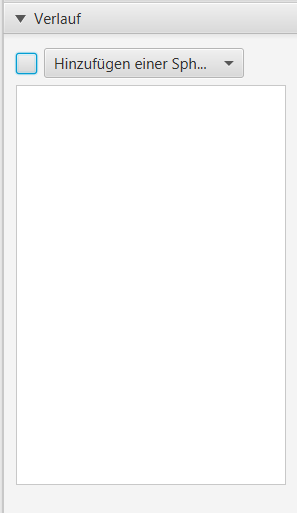
\includegraphics[height=8cm]{2_3.PNG}
\end{center}
\subsubsection{Fazit}
Die Software arbeitet wie erwartet.

\subsectiont{Mehr Sphären hinzufügen als in den Vorlage-Regeln erlaubt}{\dotfill\ok\ok\leer}
Der Bearbeiter setzt zuerst eine Sphäre links unter \texttt{Sphäre 0} und dann eine Sphäre rechts unter \texttt{Sphäre 1}. Hierbei wird erwartet, dass das Hinzufügen der ersten Sphäre erfolgreich ist, das der zweiten jedoch nicht, weil sonst die Anzahl an maximalen Sphären in den Vorlage-Regeln überschritten wird. 
\subsubsection{Notizen}
1.Test: Getestet von: Anthony Mendil. Datum: 22.02.2019 um 14:18 \\
Test negativ.\\
2.Test: Getestet von: Jacky Philipp Mach. Datum: 03.03.2019 um 19:53 \\
Test negativ.
\begin{center}
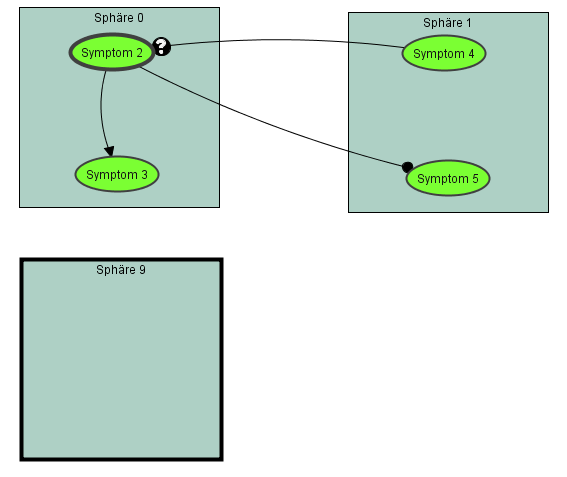
\includegraphics[height=10cm]{2_4.PNG}
\end{center}
\subsubsection{Fazit}
Die Software arbeitet wie erwartet.

\subsectiont{Abschwächende Relation hinzufügen obwohl es in den Vorlage-Regeln verboten wird}{\dotfill\ok\ok\leer}
Der Bearbeiter wählt den Relationstyp abschwächend aus und versucht von \texttt{Symptom 3} nach \texttt{Symptom 4} eine Relation zu ziehen. Zu erwarten ist, dass dies aufgrund der Vorlage-Regeln nicht erlaubt wird. 
\subsubsection{Notizen}
1.Test: Getestet von: Anthony Mendil. Datum: 22.02.2019 um 15:06 \\
Test negativ. Die Abbildung ist identisch zur vorherigen.\\
2.Test: Getestet von: Jacky Philipp Mach. Datum: 03.03.2019 um 19:55 \\
Test negativ. Die Abbildung ist identisch zur vorherigen.
\subsubsection{Fazit}
Die Software arbeitet wie erwartet.

\subsectiont{Einer Sphäre ein Symptom hinzufügen obwohl dies durch die Vorlage-Regeln verboten wird}{\dotfill\ok\ok\leer}
Der Bearbeiter versucht \texttt{Sphäre 1} rechts mittig ein Symptom hinzuzufügen. Hierbei wird erwartet, dass dies aufgrund der Vorlage-Regeln nicht erlaubt wird.
\subsubsection{Notizen}
1.Test: Getestet von: Anthony Mendil. Datum: 22.02.2019 um 16:08 \\
Test negativ. Die Abbildung ist identisch zur vorherigen.\\
2.Test: Getestet von: Jacky Philipp Mach. Datum: 03.03.2019 um 20:01 \\
Test negativ. Die Abbildung ist identisch zur vorherigen.
\subsubsection{Fazit}
Die Software arbeitet wie erwartet.

\subsectiont{Titel einer Sphäre ändern bei der es in den Vorlage-Regeln verboten wird}{\dotfill\ok\ok\leer}
Der Bearbeiter versucht den Titel von \texttt{Sphäre 0} zu ändern. Hierbei wird erwartet, dass dies aufgrund der Vorlage-Regeln nicht erlaubt wird.
\subsubsection{Notizen}
1.Test: Getestet von: Anthony Mendil. Datum: 22.02.2019 um 16:13 \\
Test negativ. Die Abbildung ist identisch zur vorherigen.\\
2.Test: Getestet von: Jacky Philipp Mach. Datum: 03.03.2019 um 20:02 \\
Test negativ. Die Abbildung ist identisch zur vorherigen.
\subsubsection{Fazit}
Die Software arbeitet wie erwartet.

\subsectiont{Style eines Symptoms ändern bei dem es in den Vorlage-Regeln verboten wird}{\dotfill\ok\ok\leer}
Der Bearbeiter versucht die Füllfarbe von \texttt{Symptom 2} zu ändern. Hierbei wird erwartet, dass dies aufgrund der Vorlage-Regeln nicht erlaubt wird.
\subsubsection{Notizen}
1.Test: Getestet von: Anthony Mendil. Datum: 22.02.2019 um 16:38 \\
Test negativ. Die Abbildung ist identisch zur vorherigen.\\
2.Test: Getestet von: Jacky Philipp Mach. Datum: 03.03.2019 um 20:04 \\
Test negativ. Die Abbildung ist identisch zur vorherigen.
\subsubsection{Fazit}
Die Software arbeitet wie erwartet.

\subsectiont{Relationsart einer Relation ändern bei der es in den Vorlage-Regeln verboten wird}{\dotfill\ok\ok\leer}
Der Bearbeiter versucht die Relationsart der Relation von \texttt{Symptom 2} nach \texttt{Symptom 3} zu einer verstärkenden Relation zu ändern. Hierbei wird erwartet, dass dies aufgrund der Vorlage-Regeln nicht erlaubt wird.
\subsubsection{Notizen}
1.Test: Getestet von: Anthony Mendil. Datum: 22.02.2019 um 16:58 \\
Test negativ. Die Abbildung ist identisch zur vorherigen.\\
2.Test: Getestet von: Jacky Philipp Mach. Datum: 03.03.2019 um 20:05 \\
Test negativ. Die Abbildung ist identisch zur vorherigen.
\subsubsection{Fazit}
Die Software arbeitet wie erwartet.

\subsectiont{Entfernen einer Sphäre mit Symptomen und Relationen}{\dotfill\ok\ok\leer}
Der Bearbeiter fügt vorerst in \texttt{Sphäre 9} ein Symptom hinzu und zieht von ihm eine verstärkende Relation zu \texttt{Symptom 5}. Anschließend entfernt er \texttt{Sphäre 9}. Es ist zu erwarten, dass mit der Sphären auch alle enthaltenden Symptome und die Relationen der Symptome gelöscht werden. 
\subsubsection{Notizen}
1.Test: Getestet von: Anthony Mendil. Datum: 22.02.2019 um 17:18 \\
Test negativ. \\
2.Test: Getestet von: Jacky Philipp Mach. Datum: 03.03.2019 um 20:06 \\
Test negativ. \\
\newpage
Nach Hinzufügen der beschriebenen Elemente: 
\begin{center}
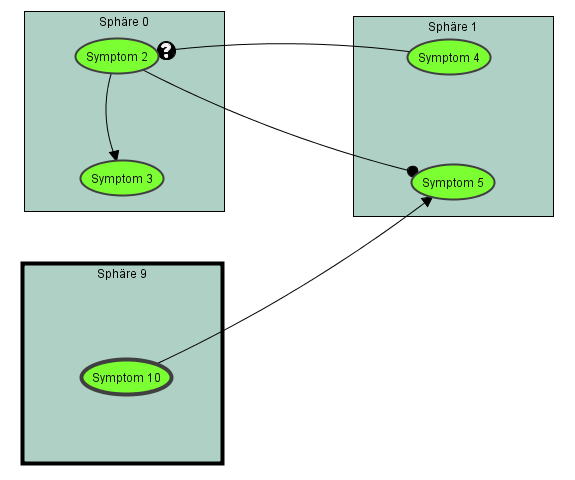
\includegraphics[height=10cm]{2_10vorher.PNG}
\end{center}
Nach Löschen der Sphäre: 
\begin{center}
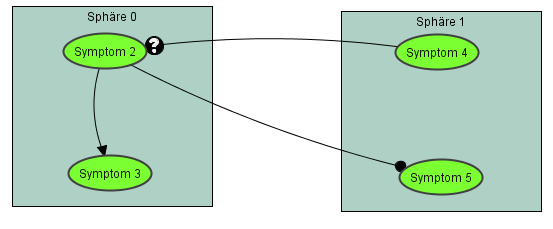
\includegraphics[height=5cm]{2_10nachher.PNG}
\end{center}
\subsubsection{Fazit}
Die Software arbeitet wie erwartet. 

\subsectiont{Rückgängig machen des Entfernens einer Sphäre mit Symptomen und Relationen}{\dotfill\XBox\ok\leer}
Der Bearbeiter betätigt den Button zum Rückgängig machen der letzten Aktion. Hierbei wird erwartet, dass die vorherige Sphäre, inklusive der ursprünglichen Symptome und Relationen wieder hinzugefügt wird. 
\subsubsection{Notizen}
1.Test: Getestet von: Anthony Mendil. Datum: 22.02.2019 um 17:48 \\
Test positiv, weil die ursprünglichen Symptome und Relationen nicht wieder hinzugefügt wurden. \\
\begin{center}
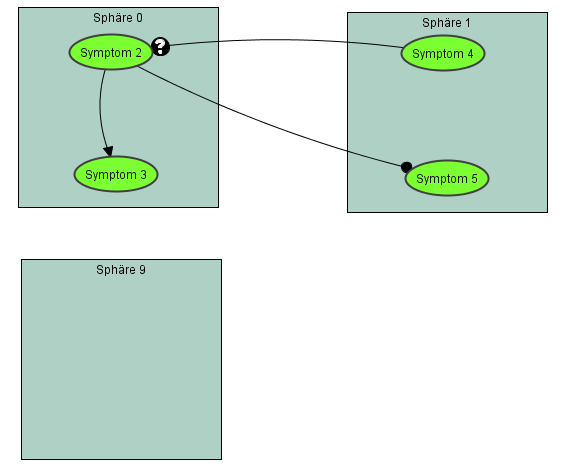
\includegraphics[height=8cm]{2_11.PNG}
\end{center}
2.Test: Getestet von: Jacky Philipp Mach. Datum: 03.03.2019 um 20:08 \\
Test negativ. \\
Nach Entfernen der Sphäre:
\begin{center}
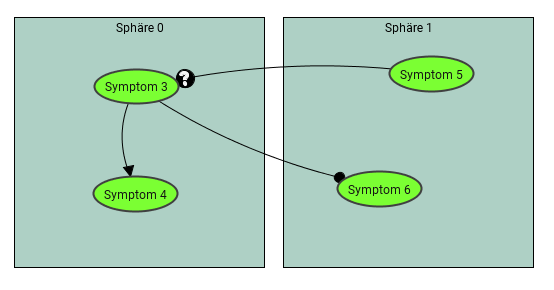
\includegraphics[height=5cm]{2_11b.png}
\end{center}
Nach Rückgängigmachen des Entfernens der Sphäre mit Symptomen und Relationen:
\begin{center}
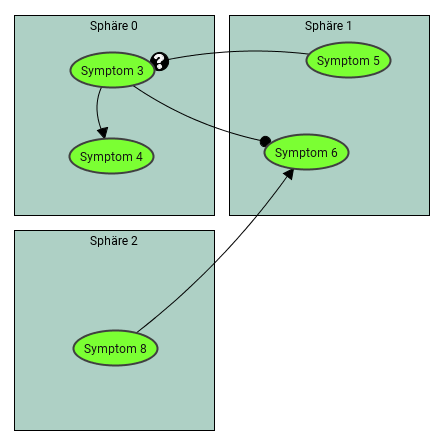
\includegraphics[height=8cm]{2_11c.png}
\end{center}
\subsubsection{Fazit}
Die an die Sphären gebundenen Elemente wurden in der Implementierung nicht beachtet. Nachdem diese hinzugefügt worden sind, arbeitet die Software wie erwartet.

\subsectiont{Vergrößern einer Sphäre}{\dotfill\ok\ok\leer}
Der Bearbeiter betätigt vorerst den Button zum Auswählen von Elementen. Anschießend macht er einen Linksklick auf \texttt{Sphäre 9} und betätigt den Button zum Vergrößern der Sphäre. Es wird erwartet, dass entsprechende Änderung auch statt findet. 
\subsubsection{Notizen}
1.Test: Getestet von: Anthony Mendil. Datum: 22.02.2019 um 18:28 \\
Test negativ.\\
2.Test: Getestet von: Jacky Philipp Mach. Datum: 03.03.2019 um 20:10 \\
Test negativ. 
\begin{center}
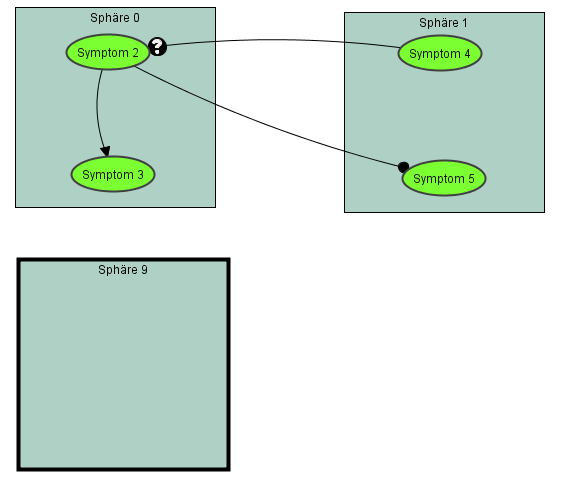
\includegraphics[height=10cm]{2_12.PNG}
\end{center}
\subsubsection{Fazit}
Die Software arbeitet wie erwartet. 

\subsectiont{Verkleinern einer Sphäre}{\dotfill\ok\ok\leer}
Vorerst entfernt der Bearbeiter \texttt{Symptom 10}. Dann macht der Bearbeiter einen Linksklick auf \texttt{Sphäre 9} und betätigt den Button zum Verkleinern der Sphäre. Es wird erwartet, dass entsprechende Änderung auch statt findet. 
\subsubsection{Notizen}
1.Test: Getestet von: Anthony Mendil. Datum: 22.02.2019 um 18:37 \\
Test negativ.\\
2.Test: Getestet von: Jacky Philipp Mach. Datum: 03.03.2019 um 20:11 \\
Test negativ. 
\begin{center}
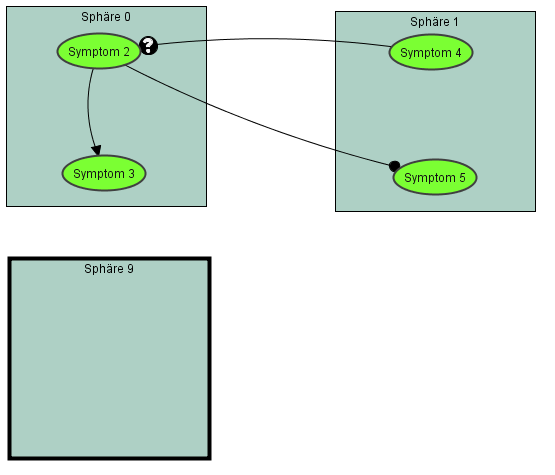
\includegraphics[height=10cm]{2_13.PNG}
\end{center}
\subsubsection{Fazit}
Die Software arbeitet wie erwartet.

\subsectiont{Ändern der Farbe einer Sphäre}{\dotfill\ok\ok\leer}
Der Bearbeiter macht einen Linksklick auf \texttt{Sphäre 9} und ändert die Farbe der Sphäre auf \texttt{Backstein} (dunkles rot). Es wird erwartet, dass die entsprechende Änderung auch statt findet. 
\subsubsection{Notizen}
1.Test: Getestet von: Anthony Mendil. Datum: 22.02.2019 um 18:37 \\
Test negativ.\\
2.Test: Getestet von: Jacky Philipp Mach. Datum: 03.03.2019 um 20:12 \\
Test negativ. 
\begin{center}
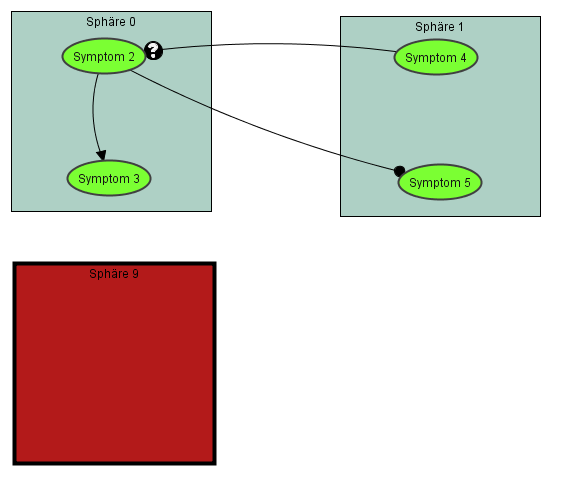
\includegraphics[height=10cm]{2_14.PNG}
\end{center}
\subsubsection{Fazit}
Die Software arbeitet wie erwartet.

\subsectiont{Ändern der Schriftart einer Sphäre}{\dotfill\ok\ok\leer}
Der Bearbeiter macht einen Linksklick auf \texttt{Sphäre 9} und ändert die Schriftart der Sphäre auf \texttt{Kalam}. Es wird erwartet, dass die entsprechende Änderung auch statt findet. 
\subsubsection{Notizen}
1.Test: Getestet von: Anthony Mendil. Datum: 22.02.2019 um 18:37 \\
Test negativ.\\
2.Test: Getestet von: Jacky Philipp Mach. Datum: 03.03.2019 um 20:13 \\
Test negativ. 
\begin{center}
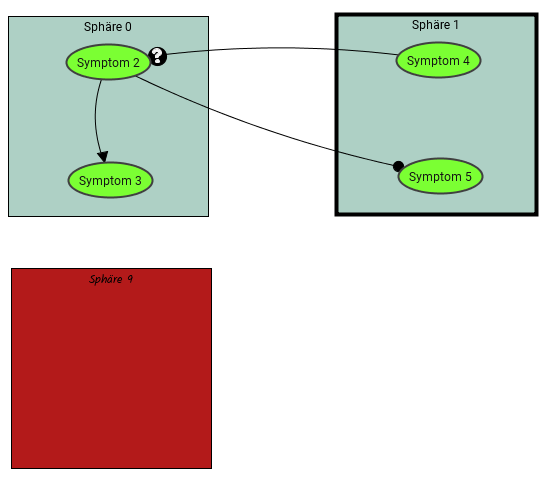
\includegraphics[height=10cm]{2_15.PNG}
\end{center}
\subsubsection{Fazit}
Die Software arbeitet wie erwartet.

\subsectiont{Verändern der Schriftgröße einer Sphäre}{\dotfill\ok\ok\leer}
Der Bearbeiter macht einen Linksklick auf \texttt{Sphäre 9} und ändert die Schriftgröße der Sphäre auf 24. Es wird erwartet, dass die entsprechende Änderung auch statt findet. 
\subsubsection{Notizen}
1.Test: Getestet von: Anthony Mendil. Datum: 22.02.2019 um 18:37 \\
Test negativ.\\
2.Test: Getestet von: Jacky Philipp Mach. Datum: 03.03.2019 um 20:13 \\
Test negativ. 
\begin{center}
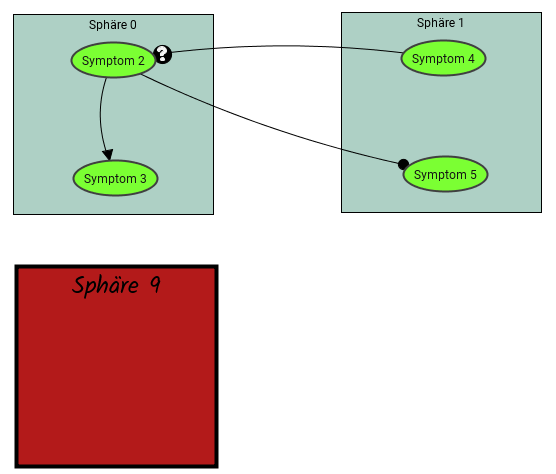
\includegraphics[height=10cm]{2_16.PNG}
\end{center}
\subsubsection{Fazit}
Die Software arbeitet wie erwartet.

\subsectiont{Sphären automatisch anordnen obwohl eine Sphäre nicht bewegt werden darf}{\dotfill\ok\ok\leer}
Der Bearbeiter versucht den Button zum automatischen Anordnen der Sphären zu betätigen. Es wird erwartet, dass dies nicht möglich ist, da das Bewegen von \texttt{Sphäre 1} in den Vorlage-Regeln verboten wird.
\subsubsection{Notizen}
1.Test: Getestet von: Anthony Mendil. Datum: 22.02.2019 um 18:37 \\
Test negativ. Die Abbildung ist identisch zur vorherigen. \\
2.Test: Getestet von: Jacky Philipp Mach. Datum: 03.03.2019 um 20:13 \\
Test negativ. Die Abbildung ist identisch zur vorherigen. 
\subsubsection{Fazit}
Die Software arbeitet wie erwartet.

\subsectiont{Sphären automatisch anordnen}{\dotfill\ok\ok\leer}
Vorerst wird in den Ersteller-Modus gewechselt um die Bewegung von \texttt{Sphäre 1} zu erlauben. Anschließend betätigt der Bearbeiter den Button zum automatischen Anordnen der Sphären. Es wird erwartet, dass die Sphären automatisch angeordnet werden und die Symptome und Relationen immer noch korrekt platziert sind.
\subsubsection{Notizen}
1.Test: Getestet von: Anthony Mendil. Datum: 22.02.2019 um 18:37 \\
Test negativ.\\
2.Test: Getestet von: Jacky Philipp Mach. Datum: 03.03.2019 um 20:13 \\
Test negativ. 
\begin{center}
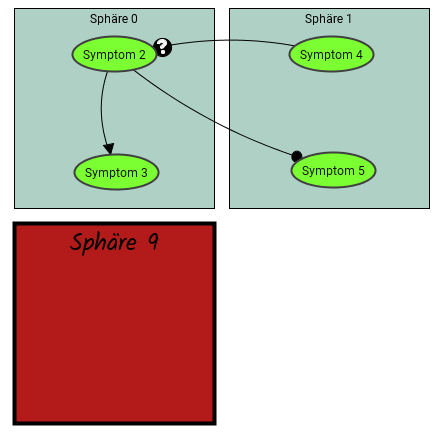
\includegraphics[height=10cm]{2_17.PNG}
\end{center}
\subsubsection{Fazit}
Die Software arbeitet wie erwartet.

\subsectiont{Rückgängig machen der automatischen Anordnung von Sphären}{\dotfill\ok\ok\leer}
Der Bearbeiter betätigt den Button zum Rückgängigmachen der letzten Aktion. Es wird erwartet, dass die Sphären mit ihren Knoten und den Relationen wieder an ihre vorherige Positionen bewegt werden.
\subsubsection{Notizen}
1.Test: Getestet von: Anthony Mendil. Datum: 22.02.2019 um 18:37 \\
Test negativ.\\
2.Test: Getestet von: Jacky Philipp Mach. Datum: 03.03.2019 um 20:15 \\
Test negativ. 
\begin{center}
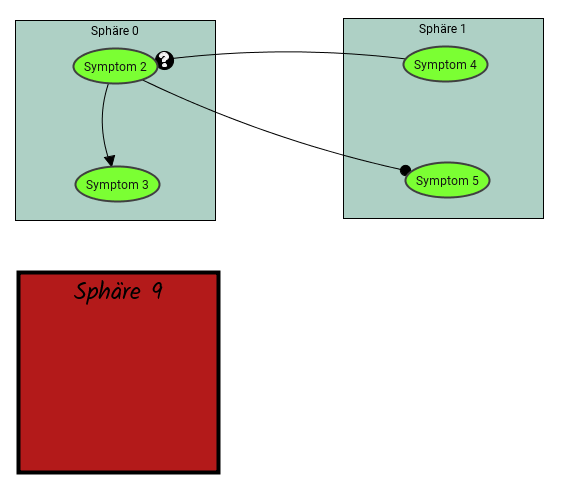
\includegraphics[height=10cm]{2_18.PNG}
\end{center}
\subsubsection{Fazit}
Die Software arbeitet wie erwartet.

\subsectiont{Bewegen einer Sphäre auf eine andere}{\dotfill\ok\ok\leer}
Der Bearbeiter versucht \texttt{Sphäre 9} auf \texttt{Sphäre 0} zu bewegen. Hierbei wird erwartet, dass \texttt{Sphäre 9} auf ihre ursprüngliche Position zurück bewegt wird und \texttt{Sphäre 0} unverändert bleibt.   
\subsubsection{Notizen}
1.Test: Getestet von: Anthony Mendil. Datum: 22.02.2019 um 18:37 \\
Test negativ. Die Abbildung ist identisch zur vorherigen. \\
2.Test: Getestet von: Jacky Philipp Mach. Datum: 03.03.2019 um 20:16 \\
Test negativ. Die Abbildung ist identisch zur vorherigen.
\subsubsection{Fazit}
Die Software arbeitet wie erwartet.

\subsection*{Symptome}

\subsectiont{Entfernen eines Symptoms, das Relationen hat}{\dotfill\ok\ok\leer}
Der Bearbeiter fügt vorerst in \texttt{Sphäre 9} ein Symptom hinzu und zieht von ihm eine verstärkende Relation zu \texttt{Symptom 5} und eine von \texttt{Symptom 3} zum hinzugefügten Symptom. Anschließend entfernt er das soeben hinzugefügte Symptom nachdem er es mit einem Linksklick ausgewählt hat. Es ist zu erwarten, dass mit dem Symptom auch alle ausgehenden und eingehenden Relationen des gelöschten Symptoms entfernt werden. 
\subsubsection{Notizen}
1.Test: Getestet von: Anthony Mendil. Datum: 23.02.2019 um 10:58 \\
Test negativ. \\
2.Test: Getestet von: Jacky Philipp Mach. Datum: 03.03.2019 um 20:18 \\
Test negativ.\\ \\
Nach dem Hinzufügen der beschriebenen Elemente: 
\begin{center}
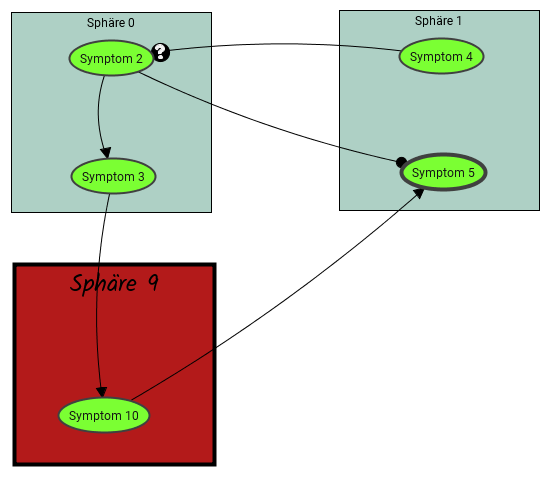
\includegraphics[height=10cm]{2_20korrektvorher.PNG}
\end{center}
\newpage
Nach dem Löschen der Sphäre: 
\begin{center}
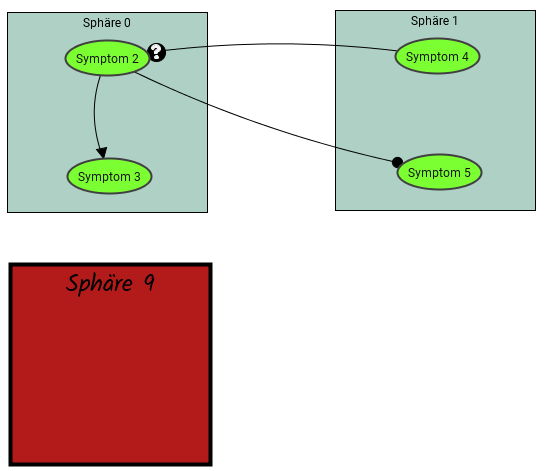
\includegraphics[height=10cm]{2_20korrektnachher.PNG}
\end{center}
\subsubsection{Fazit}
Die Software arbeitet wie erwartet. 

\subsectiont{Rückgängig machen des Entfernens eines \\Symptoms mit Relationen}{\dotfill\XBox\ok\leer}
Der Bearbeiter betätigt den Button zum Rückgängigmachen der letzten Aktion. Hierbei wird erwartet, dass das vorherige Symptom, inklusive der ursprünglichen Relationen wieder hinzugefügt wird. 
\subsubsection{Notizen}
1.Test: Getestet von: Anthony Mendil. Datum: 23.02.2019 um 11:33 \\
Test positiv, weil die ursprünglichen Symptome und Relationen nicht wieder hinzugefügt wurden. Der Graph verändert sich nicht. \\
2.Test: Getestet von: Anthony Mendil. Datum: 23.02.2019 um 20:18 \\
Test negativ.
\begin{center}
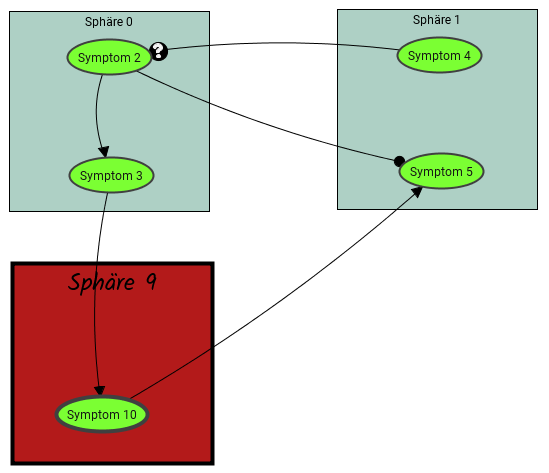
\includegraphics[height=10cm]{2_21.PNG}
\end{center}
\subsubsection{Fazit}
Die Relationen, welche eine eingehende oder ausgehende Relation des zu löschenden Symptoms ist wurde in der Implementierung nicht beachtet. Nachdem die Semantik dazu implementiert wurde arbeitet die Software wie erwartet. 

\subsectiont{Entfernen mehrere Symptome ohne Relationen}{\dotfill\XBox\ok\leer}
Zunächst entfernt der Bearbeiter alle Relationen von \texttt{Symptom 10}, verschiebt es ein wenig nach links und fügt \texttt{Sphäre 9} ein weiteres Symptom rechts von \texttt{Symptom 10} hinzu. 
Durch gedrückt halten von Umschalten und Linksklicks auf die soeben erwähnten Symptome wählt der Bearbeiter mehrere Symptome aus. Das rechte Symptom ist nach dem Hinzufügen bereits ausgewählt, weshalb auf die soeben beschriebene Weise nur noch das linke Symptom der Auswahl hinzugefügt werden muss. Anschließend betätigt er den Button zum Löschen der Symptome. Hierbei wird erwartet, dass alle ausgewählten Symptome gelöscht werden. 
\subsubsection{Notizen}
1.Test: Getestet von: Anthony Mendil. Datum: 23.02.2019 um 11:39 \\
Test positiv, weil nur eins der ausgewählten Symptome entfernt wurde. \\
Nach Hinzufügen der beiden Symptome: 
\begin{center}
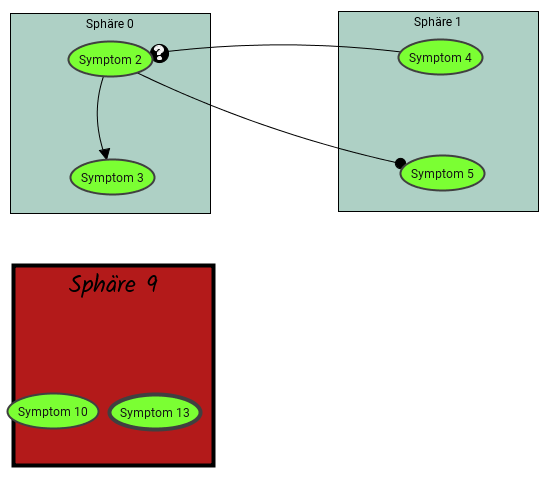
\includegraphics[height=10cm]{2_22vorher.PNG}
\end{center}
Nach Betätigen des Buttons zum Entfernen der Symptome: 
\begin{center}
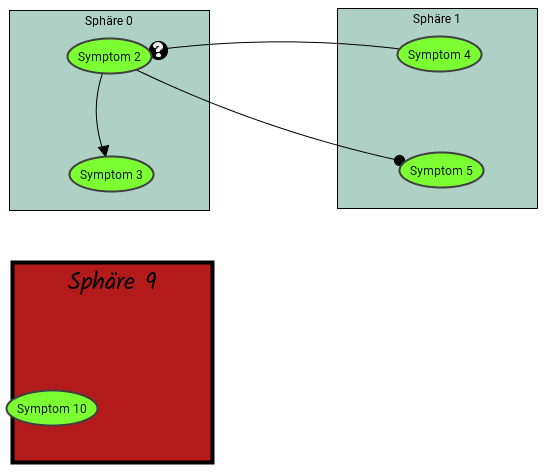
\includegraphics[height=10cm]{2_22nachher.PNG}
\end{center}
2.Test: Getestet von: Anthony Mendil. Datum: 23.02.2019 um 20:26 \\
Test negativ. \\
Nach Hinzufügen der beiden Symptome: 
\begin{center}
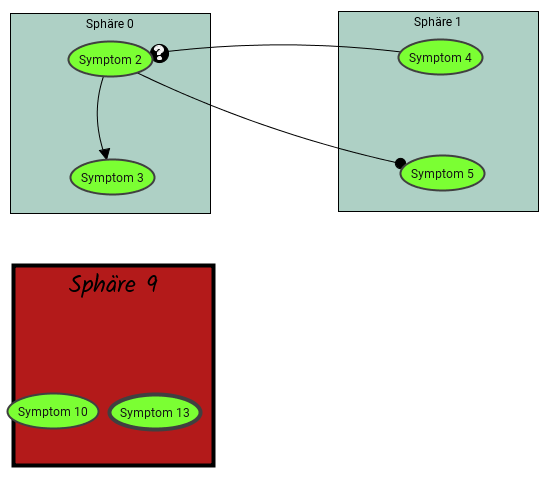
\includegraphics[height=10cm]{2_22vorher.PNG}
\end{center}
Nach Betätigen des Buttons zum Entfernen der Symptome: 
\begin{center}
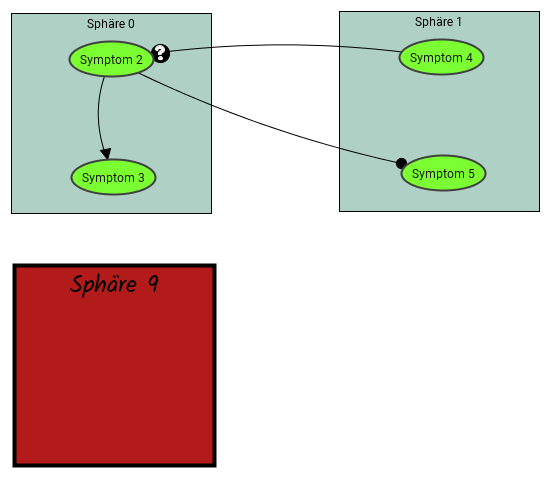
\includegraphics[height=10cm]{2_22.PNG}
\end{center}
\subsubsection{Fazit}
Die Menge der ausgewählten Symptome wurde in der jeweiligen Action nicht richtig iteriert. Nachdem dieser Fehler behoben wurde, arbeitet die Software nun wie erwartet.

\subsectiont{Vergrößern eines Symptoms}{\dotfill\ok\ok\leer}
Der Bearbeiter fügt links mittig in \texttt{Sphäre 9} eine Symptom hinzu und betätigt den Button zum Vergrößern des Symptoms zehn mal. Hierbei wird erwartet, dass entsprechende Änderungen an dem Knoten vorgenommen werden.
\subsubsection{Notizen}
1.Test: Getestet von: Anthony Mendil. Datum: 23.02.2019 um 12:32 \\
Test negativ.\\
2.Test: Getestet von: Jacky Philipp Mach. Datum: 04.03.2019 um 12:14 \\
Test negativ.
\begin{center}
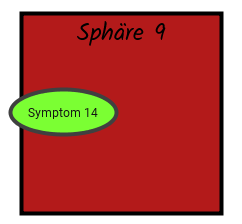
\includegraphics[height=5cm]{2_23.PNG}
\end{center}
\subsubsection{Fazit}
Die Software arbeitet wie erwartet.

\subsectiont{Verkleinern eines Symptoms}{\dotfill\ok\ok\leer}
Der Bearbeiter wählt \texttt{Symptom 10} aus und betätigt den Button zum Verkleinern des Symptoms zehn mal. Hierbei wird erwartet, dass entsprechende Änderungen an dem Knoten vorgenommen werden.
\subsubsection{Notizen}
1.Test: Getestet von: Anthony Mendil. Datum: 23.02.2019 um 12:34 \\
Test negativ.\\
2.Test: Getestet von: Jacky Philipp Mach. Datum: 04.03.2019 um 12:15 \\
Test negativ.
\begin{center}
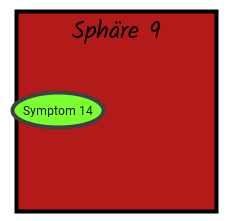
\includegraphics[height=5cm]{2_24.PNG}
\end{center}
\subsubsection{Fazit}
Die Software arbeitet wie erwartet.

\subsectiont{Ändern der Füllfarbe eines Symptoms}{\dotfill\ok\ok\leer}
Der Bearbeiter wählt \texttt{Symptom 10} aus und ändert die Füllfarbe des Symptoms zu Kornblumenblau. Hierbei wird erwartet, dass entsprechende Änderungen an dem Knoten vorgenommen werden.
\subsubsection{Notizen}
1.Test: Getestet von: Anthony Mendil. Datum: 23.02.2019 um 12:36 \\
Test negativ.\\
2.Test: Getestet von: Jacky Philipp Mach. Datum: 04.03.2019 um 12:15 \\
Test negativ.
\begin{center}
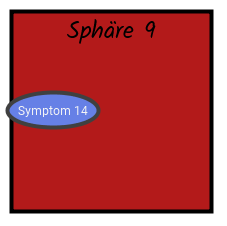
\includegraphics[height=5cm]{2_25.PNG}
\end{center}
\subsubsection{Fazit}
Die Software arbeitet wie erwartet.

\subsectiont{Ändern der Randfarbe eines Symptoms}{\dotfill\ok\ok\leer}
Der Bearbeiter wählt \texttt{Symptom 10} aus und ändert die Randfarbe des Symptoms zu Goldrute. Hierbei wird erwartet, dass entsprechende Änderungen an dem Knoten vorgenommen werden.
\subsubsection{Notizen}
1.Test: Getestet von: Anthony Mendil. Datum: 23.02.2019 um 12:39 \\
Test negativ.\\
2.Test: Getestet von: Jacky Philipp Mach. Datum: 04.03.2019 um 12:16 \\
Test negativ.
\begin{center}
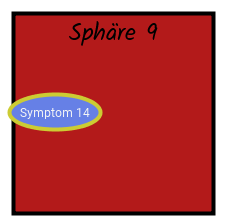
\includegraphics[height=5cm]{2_26.PNG}
\end{center}
\subsubsection{Fazit}
Die Software arbeitet wie erwartet.

\subsectiont{Ändern der Form eines Symptoms}{\dotfill\ok\ok\leer}
Der Bearbeiter wählt \texttt{Symptom 10} aus und ändert die Form des Symptoms zu rechteckig. Hierbei wird erwartet, dass entsprechende Änderungen an dem Knoten vorgenommen werden.
\subsubsection{Notizen}
1.Test: Getestet von: Anthony Mendil. Datum: 23.02.2019 um 14:12 \\
Test negativ.\\
2.Test: Getestet von: Jacky Philipp Mach. Datum: 04.03.2019 um 12:16 \\
Test negativ.
\begin{center}
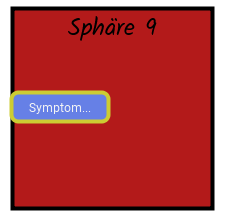
\includegraphics[height=5cm]{2_27.PNG}
\end{center}
\subsubsection{Fazit}
Die Software arbeitet wie erwartet.

\subsectiont{Automatisches Anordnen der Symptome obwohl ein Symptom nicht bewegt werden darf}{\dotfill\ok\ok\leer}
Der Bearbeiter versucht den Button zum automatischen Anordnen der Symptome zu betätigen. Hierbei wird erwartet, dass dies nicht erlaubt wird, da das Bewegen von \texttt{Symptom 3} in den Vorlage-Regeln verboten wird. 
\subsubsection{Notizen}
1.Test: Getestet von: Anthony Mendil. Datum: 23.02.2019 um 14:18 \\
Test negativ. Die Abbildung ist identisch zur vorherigen. \\
2.Test: Getestet von: Jacky Philipp Mach. Datum: 04.03.2019 um 12:14 \\
Test negativ. Die Abbildung ist identisch zur vorherigen. 
\subsubsection{Fazit}
Die Software arbeitet wie erwartet.

\subsectiont{Automatisches Anordnen der Symptome}{\dotfill\ok\ok\leer}
Vorerst wird in den Ersteller-Modus gewechselt, um das Bewegen von \texttt{Symptom 3} zu erlauben. Anschließend wird wieder in den Bearbeiter-Modus gewechselt. Der Bearbeiter betätigt den Button zum automatischen Anordnen der Symptome. Hierbei wird erwartet, dass die Symptome in den Sphären automatisch angeordnet werden. 
\subsubsection{Notizen}
1.Test: Getestet von: Anthony Mendil. Datum: 23.02.2019 um 14:18 \\
Test negativ.\\
2.Test: Getestet von: Jacky Philipp Mach. Datum: 04.03.2019 um 12:14 \\
Test negativ.
\begin{center}
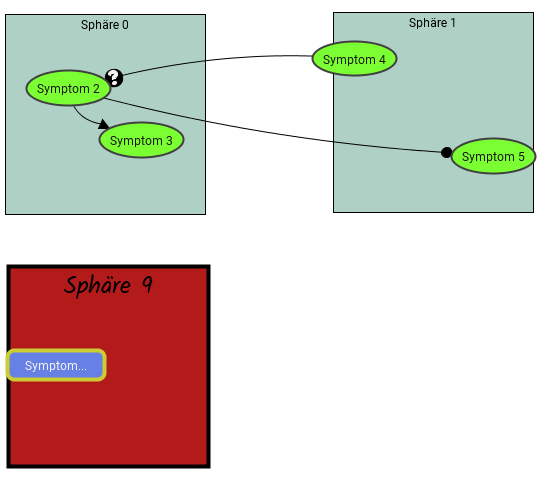
\includegraphics[height=10cm]{2_28.PNG}
\end{center}
\subsubsection{Fazit}
Die Software arbeitet wie erwartet.

\subsectiont{Ändern der Schriftart mehrerer Symptome, wobei dies durch die Vorlage-Regeln nicht bei allen erlaubt wird}{\dotfill\ok\ok\leer}
Der Bearbeiter wählt \texttt{Symptom 2}, \texttt{Symptom 4} und \texttt{Symptom 5} aus und ändert die Schriftart der Symptome zu \texttt{Kalam}. Hierbei wird erwartet, dass die Schriftart von  \texttt{Symptom 2} und \texttt{Symptom 4} entsprechend verändert wird, während die Schriftart von \texttt{Symptom 5} gleich bleibt, da deren Änderung in den Vorlage-Regeln verboten wurde (Schriftart wird mit unter \texttt{Style} aufgefasst).  
\subsubsection{Notizen}
1.Test: Getestet von: Anthony Mendil. Datum: 23.02.2019 um 14:46 \\
Test negativ.\\
2.Test: Getestet von: Jacky Philipp Mach. Datum: 04.03.2019 um 12:16 \\
Test negativ.
\begin{center}
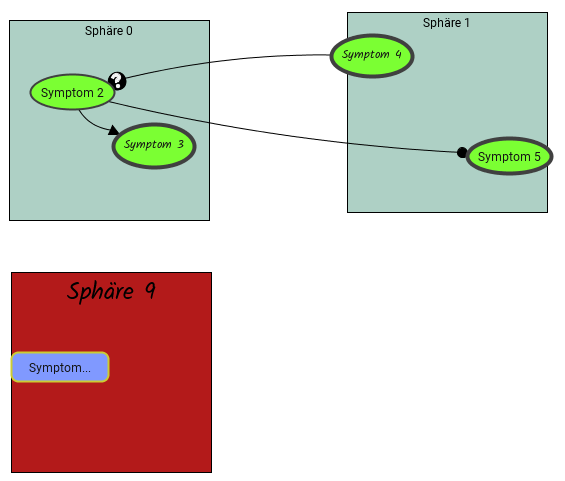
\includegraphics[height=10cm]{2_29.PNG}
\end{center}
\subsubsection{Fazit}
Die Software arbeitet wie erwartet.

\subsectiont{Ändern der Schriftgröße eines Symptoms}{\dotfill\ok\ok\leer}
Der Bearbeiter wählt \texttt{Symptom 5} aus und ändert seine Schriftgröße zu 24. Hierbei wird erwartet, die Schrift des Symptoms größer wird und die Größe des Symptoms ebenfalls so wächst, dass die Beschriftung noch komplett angezeigt wird. 
\subsubsection{Notizen}
1.Test: Getestet von: Anthony Mendil. Datum: 23.02.2019 um 14:50 \\
Test negativ.\\
2.Test: Getestet von: Jacky Philipp Mach. Datum: 04.03.2019 um 12:19 \\
Test negativ.
\begin{center}
\includegraphics[height=10cm]{2_30.PNG}
\end{center}
\subsubsection{Fazit}
Die Software arbeitet wie erwartet.

\subsectiont{Bewegen eines Symptoms in eine andere Sphäre}{\dotfill\ok\ok\leer}
Der Bearbeiter bewegt \texttt{Symptom 5} in \texttt{Sphäre 9}. Hierbei wird erwartet, dass das Symptom nach \texttt{Sphäre 9} verschoben wird und die eingehende Relation des Symptoms mitwandert. 
\subsubsection{Notizen}
1.Test: Getestet von: Anthony Mendil. Datum: 23.02.2019 um 14:33 \\
Test negativ.\\
2.Test: Getestet von: Jacky Philipp Mach. Datum: 04.03.2019 um 12:22 \\
Test negativ.
\begin{center}
\includegraphics[height=10cm]{2_31.PNG}
\end{center}
\subsubsection{Fazit}
Die Software arbeitet wie erwartet.

\subsectiont{Bewegen eines Symptoms an eine Stelle \\an der keine Sphäre liegt}{\dotfill\ok\ok\leer}
Der Bearbeiter bewegt \texttt{Symptom 5} rechts neben \texttt{Sphäre 9}. Hierbei wird erwartet, dass das Symptom inklusive seiner eingehenden Relation wieder an ihre ursprünglichen Positionen zurück springen. 
\subsubsection{Notizen}
1.Test: Getestet von: Anthony Mendil. Datum: 23.02.2019 um 14:37 \\
Test negativ.\\
2.Test: Getestet von: Jacky Philipp Mach. Datum: 04.03.2019 um 12:22 \\
Test negativ.
\begin{center}
\includegraphics[height=10cm]{2_31.PNG}
\end{center}
\subsubsection{Fazit}
Die Software arbeitet wie erwartet.

\subsectiont{Verändern der Farbe einer Relation}{\dotfill\ok\ok\leer}
Vorerst fügt der Bearbeiter \texttt{Sphäre 1} ein Symptom hinzu (Schriftart: Roboto) und zieht eine verstärkende Relation von \texttt{Symptom 4} zum eben erstellten. Anschließend wählt er die Relation aus und ändern ihre Farbe zu \texttt{Königsblau}. Hierbei wird erwartet, dass entsprechende Änderung stattfindet. 
\subsubsection{Notizen}
1.Test: Getestet von: Anthony Mendil. Datum: 24.02.2019 um 15:28 \\
Test negativ. \\
2.Test: Getestet von: Jacky Philipp Mach. Datum: 04.03.2019 um 12:24 \\
Test negativ.\\
\newpage
Nach Hinzufügen des Symptoms und der Relation: 
\begin{center}
\includegraphics[height=9.5cm]{3_33vorher.PNG}
\end{center}
Nach Ändern der Farbe der Relation von \texttt{Symptom 4} nach \texttt{Symptom 15} :
\begin{center}
\includegraphics[height=9.5cm]{3_33.PNG}
\end{center}
\subsubsection{Fazit}
Die Software arbeitet wie erwartet.

\subsectiont{Verändern der Linienart einer Relation}{\dotfill\ok\ok\leer}
Der Bearbeiter wählt die Relation von \texttt{Symptom 4} nach \texttt{Symptom 15} aus und ändern ihre Linienart zu gepunktet. Hierbei wird erwartet, dass entsprechende Änderung stattfindet. 
\subsubsection{Notizen}
1.Test: Getestet von: Anthony Mendil. Datum: 24.02.2019 um 16:01 \\
Test negativ.\\
2.Test: Getestet von: Jacky Philipp Mach. Datum: 04.03.2019 um 12:25 \\
Test negativ.
\begin{center}
\includegraphics[height=10cm]{3_34.PNG}
\end{center}
\subsubsection{Fazit}
Die Software arbeitet wie erwartet.

\subsectiont{Zusammenfassung gleicher Pfeilspitzen}{\dotfill\ok\ok\leer}
Der Bearbeiter fügt vorerst zu \texttt{Sphäre 0} oben rechts ein Symptom hinzu und zieht von ihm aus eine verstärkende Relation zu \texttt{Symptom 15}. Hierbei wird erwartet, dass die Pfeilspitzen der Relation mit der Relation von \texttt{Symptom 18} nach \texttt{Symptom 15} zusammengefasst wird, da es sich um die gleiche Pfeilspitze handelt.
\subsubsection{Notizen}
1.Test: Getestet von: Anthony Mendil. Datum: 24.02.2019 um 16:28 \\
Test negativ. \\
2.Test: Getestet von: Jacky Philipp Mach. Datum: 04.03.2019 um 12:28 \\
Test negativ.\\
Nach Hinzufügen des Symptoms und der Relation: 
\begin{center}
\includegraphics[height=10cm]{3_35.PNG}
\end{center}
\subsubsection{Fazit}
Die Software arbeitet wie erwartet.

\subsectiont{Verändern der Relationsart einer Relation}{\dotfill\ok\ok\leer}
Damit folgende Aktion möglich ist, muss vorerst in den Ersteller-Modus gewechselt werden um abschwächende Relationen zu erlauben. Anschließend wählt der Bearbeiter die Relation von \texttt{Symptom 4} nach \texttt{Symptom 15} aus und ändert die Relationsart zu abschwächend. Hierbei wird einerseits erwartet, dass der Relationstyp der Relation geändert wird und andererseits, dass die Pfeilspitzen der Relation nicht mehr mit der Relation von \texttt{Symptom 18} nach \texttt{Symptom 15} zusammengefasst wird, da es sich nach der Änderung nicht mehr um die gleiche Pfeilspitze handelt.
\subsubsection{Notizen}
1.Test: Getestet von: Anthony Mendil. Datum: 24.02.2019 um 17:04 \\
Test negativ. \\
2.Test: Getestet von: Jacky Philipp Mach. Datum: 04.03.2019 um 12:30 \\
Test negativ.
\begin{center}
\includegraphics[height=10cm]{3_36.PNG}
\end{center}
\subsubsection{Fazit}
Die Software arbeitet wie erwartet.

\subsectiont{Hinzufügen von Ankerpunkten}{\dotfill\ok\ok\leer}
Vorerst betätigt der Bearbeiter den Button zum Einblenden/Ausblenden von Ankerpunkten. Anschließend bewegt er von der Relation von \texttt{Symptom 4} nach \texttt{Symptom 15} die Stelle, an dem die Kante zu \texttt{Symptom 4} verläuft, indem er den Rechtsklick (gedrückt halten und bewegen) nahe des genannten Symptoms macht. Selbiges macht er nahe \texttt{Symptom 15} um dort selbiges zu bewirken. Bei den Aktionen wird erwartet, dass jeweils ein Ankerpunkt erstellt wird.
\subsubsection{Notizen}
1.Test: Getestet von: Anthony Mendil. Datum: 24.02.2019 um 18:46 \\
Test negativ.\\
2.Test: Getestet von: Jacky Philipp Mach. Datum: 04.03.2019 um 12:33 \\
Test negativ.
\begin{center}
\includegraphics[height=10cm]{3_37.PNG}
\end{center}
\subsubsection{Fazit}
Die Software arbeitet wie erwartet.

\subsectiont{Ankerpunkte ausblenden}{\dotfill\ok\ok\leer}
Der Bearbeiter betätigt erneut den Button zum Einblenden/Ausblenden von Ankerpunkten. Hierbei wird erwartet, dass die vorerst angezeigten Ankerpunkte ausgeblendet werden. 
\subsubsection{Notizen}
1.Test: Getestet von: Anthony Mendil. Datum: 24.02.2019 um 18:53 \\
Test negativ.\\
2.Test: Getestet von: Jacky Philipp Mach. Datum: 04.03.2019 um 12:34 \\
Test negativ.
\begin{center}
\includegraphics[height=10cm]{3_38.PNG}
\end{center}
\subsubsection{Fazit}
Die Software arbeitet wie erwartet.

\subsectiont{Ankerpunkte einblenden}{\dotfill\ok\ok\leer}
Der Bearbeiter betätigt erneut den Button zum Einblenden/Ausblenden von Ankerpunkten. Hierbei wird erwartet, dass die vorerst ausgeblendeten Ankerpunkte eingeblendet werden. 
\subsubsection{Notizen}
1.Test: Getestet von: Anthony Mendil. Datum: 24.02.2019 um 19:24 \\
Test negativ.\\
2.Test: Getestet von: Jacky Philipp Mach. Datum: 04.03.2019 um 12:35 \\
Test negativ.
\begin{center}
\includegraphics[height=10cm]{3_39.PNG}
\end{center}
\subsubsection{Fazit}
Die Software arbeitet wie erwartet.

\subsectiont{Entfernen mehrerer Relationen}{\dotfill\ok\ok\leer}
Der Bearbeiter wählt mit Umschalten und Linksklick die Relation von \texttt{Symptom 18} nach \texttt{Symptom 15} und die von \texttt{Symptom 4} nach \texttt{Symptom 15} aus und betätigt den Button zum Entfernen von Relationen. Hierbei ist zu erwarten, dass beide Relationen inklusive der Ankerpunkte entfernt werden. 
\subsubsection{Notizen}
1.Test: Getestet von: Anthony Mendil. Datum: 24.02.2019 um 19:17 \\
Test negativ. \\
2.Test: Getestet von: Jacky Philipp Mach. Datum: 04.03.2019 um 12:37 \\
Test negativ.
\begin{center}
\includegraphics[height=10cm]{3_40.PNG}
\end{center}
\subsubsection{Fazit}
Die Software arbeitet wie erwartet.

\subsectiont{Rückgängig machen des Entfernens mehrerer Relationen mit Ankerpunkten}{\dotfill\ok\ok\leer}
Der Bearbeiter betätigt den Button zum Rückgängigmachen der letzten Aktion. Hierbei wird erwartet, dass die vorher entfernten Relationen inklusive ihrer Ankerpunkte wieder hinzugefügt werden.
\subsubsection{Notizen}
1.Test: Getestet von: Anthony Mendil. Datum: 24.02.2019 um 19:35 \\
Test negativ.\\
2.Test: Getestet von: Jacky Philipp Mach. Datum: 04.03.2019 um 12:39 \\
Test negativ.
\begin{center}
\includegraphics[height=10cm]{3_41.PNG}
\end{center}
\subsubsection{Fazit}
Die Software arbeitet wie erwartet.

\subsectiont{Bewegen eines Symptoms, bei dem eine \\Relation Ankerpunkte hat}{\dotfill\ok\ok\leer}
Der Bearbeiter bewegt \texttt{Symptom 4} innerhalb seiner Sphäre weiter nach rechts. Hierbei wird erwarten, dass die Punkte, an denen die Relation von \texttt{Symptom 4} nach \texttt{Symptom 15} an den eben genannten Symptomen andockt nicht verschoben werden, da die Relation Ankerpunkte hat. Ohne Ankerpunkte würden sie sich der Verschiebung anpassen. 
\subsubsection{Notizen}
1.Test: Getestet von: Anthony Mendil. Datum: 25.02.2019 um 12:07 \\
Test negativ.\\
2.Test: Getestet von: Jacky Philipp Mach. Datum: 04.03.2019 um 12:41 \\
Test negativ.
\begin{center}
\includegraphics[height=10cm]{3_42.PNG}
\end{center}
\subsubsection{Fazit}
Die Software arbeitet wie erwartet.

\subsectiont{Bei angezeigten Ankerpunkten in den Analyse-Modus wechseln}{\dotfill\XBox\ok\leer}
Der Bearbeiter wechselt in den Analyse-Modus. Hierbei wird erwartet, dass alle im Bearbeiter-Modus angezeigten Ankerpunkte im Analyse-Modus nicht mehr angezeigt werden. 
\subsubsection{Notizen}
1.Test: Getestet von: Anthony Mendil. Datum: 25.02.2019 um 13:01 \\
Test positiv, weil noch ein Ankerpunkt angezeigt wird. Genauer gesagt wird bei der Relation von \texttt{Symptom 4} nach \texttt{Symptom 15} der Ankerpunkt an \texttt{Symptom 4} noch angezeigt. \\
\begin{center}
\includegraphics[height=10cm]{3_43.PNG}
\end{center}
2.Test: Getestet von: Jacky Philipp Mach. Datum: 05.03.2019 um 14:11 \\
Test negativ. \\\\
\newpage
Vor dem Wechsel in den Analyse-Modus:
\begin{center}
\includegraphics[height=9.5cm]{3_45vorher.png}
\end{center}
Nach dem Wechsel in den Analyse-Modus:
\begin{center}
\includegraphics[height=9.5cm]{3_45nachher.png}
\end{center}
\subsubsection{Fazit}
Nach dem ersten Test wurde ein Wahrheitswert in \texttt{Values} hinzugefügt, der dazu führt, dass auch der betroffene Ankerpunkt nicht mehr angezeigt wird, wenn man den Modus wechselt. Beim zweiten Test arbeitet die Software wie erwartet.

\subsectiont{Änderung der Beschriftung eines Symptoms}{\dotfill\ok\ok\leer}
Vorerst wird wieder in den Bearbeiter-Modus gewechselt. Mithilfe eines Rechtsklicks auf \texttt{Symptom 15} und drücken auf \texttt{Titel} öffnet der Bearbeiter ein Fenster zur Eingabe der Beschriftung des Symptoms in Deutsch und Englisch. Dann gibt er in dem Feld für die deutsche Beschriftung \texttt{Individualisierung}  und in dem für die englische Beschriftung \texttt{Individualization} ein und drückt auf \texttt{Speichern}. Hierbei wird erwartet, dass in dem Symptom nun \texttt{Individualisierung} steht. 
\subsubsection{Notizen}
1.Test: Getestet von: Anthony Mendil. Datum: 25.02.2019 um 14:59 \\
Test negativ. \\
2.Test: Getestet von: Jacky Philipp Mach. Datum: 04.03.2019 um 13:01 \\
Test negativ.\\\\
Nach dem Klick auf Titel: 
\begin{center}
\includegraphics[height=9.5cm]{3_44oeffnen.PNG}
\end{center}
Nach der Eingabe der Beschriftungen:
\begin{center}
\includegraphics[height=9.5cm]{3_44eingabe.PNG}
\end{center}
Nach den Drücken auf \texttt{Speichern}:
\begin{center}
\includegraphics[height=9.5cm]{3_44speichern.PNG}
\end{center}
\subsubsection{Fazit}
Die Software arbeitet wie erwartet.

\subsectiont{Ändern der Sprache des Graphen}{\dotfill\ok\ok\leer}
Der Bearbeiter geht auf \texttt{Optionen}, unter \texttt{erweiterte Spracheinstellungen}, \texttt{Sprache des Graphen} und dann auf \texttt{Englisch}. Hierbei wird erwartet, dass die Sprache aller Graph-Elemente auf Englisch gestellt werden.
\subsubsection{Notizen}
1.Test: Getestet von: Anthony Mendil. Datum: 25.02.2019 um 15:08 \\
Test negativ. \\
2.Test: Getestet von: Jacky Philipp Mach. Datum: 04.03.2019 um 13:03 \\
Test negativ.
\begin{center}
\includegraphics[height=10cm]{3_45.PNG}
\end{center}
\subsubsection{Fazit}
Die Software arbeitet wie erwartet.

\subsectiont{Bewegen eines Symptoms auf ein anderes Symptom}{\dotfill\ok\ok\leer} 
Der Bearbeiter bewegt \texttt{Individualization} auf \texttt{Symptom 4}. Hierbei wird erwartet, dass das bewegte Symptom wieder auf seine vorherige Position zurück springt. 
\subsubsection{Notizen}
1.Test: Getestet von: Anthony Mendil. Datum: 25.02.2019 um 15:13 \\
Test negativ. Die Abbildung ist identisch zur vorherigen. \\
2.Test: Getestet von: Jacky Philipp Mach. Datum: 04.03.2019 um 13:03 \\
Test negativ. Die Abbildung ist identisch zur vorherigen. 
\subsubsection{Fazit}
Die Software arbeitet wie erwartet.

\subsectiont{Änderung der Beschriftung eines Symptoms zu einer bereits existierenden Beschriftung}{\dotfill\ok\ok\leer}
Vorerst wird die Sprache des Graphen wieder auf Deutsch gestellt. Anschließend macht der Bearbeiter einen Rechtsklick auf \texttt{Symptom 4} und drückt auf \texttt{Titel}. Dort versucht er die deutsche Beschriftung des Symptoms zu \texttt{Individualisierung } zu ändern. Das Leerzeichen nach \texttt{Individualisierung} ist wichtig um zu testen, ob die Aktion trotz Leerzeichen verboten wird. Hierbei wird erwartet, dass dies nicht erlaubt wird, da bereits ein anderes Symptom diese Beschriftung hat. 
\subsubsection{Notizen}
1.Test: Getestet von: Anthony Mendil. Datum: 25.02.2019 um 15:20 \\
Test negativ. \\
2.Test: Getestet von: Jacky Philipp Mach. Datum: 04.03.2019 um 13:05 \\
Test negativ.\\\\
\newpage
Nach den Klick auf Titel: 
\begin{center}
\includegraphics[height=9.5cm]{3_46vorher.PNG}
\end{center}
Nach Eingabe der deutschen Beschriftung:
\begin{center}
\includegraphics[height=9.5cm]{3_46nachher.PNG}
\end{center}
\subsubsection{Fazit}
Die Software arbeitet wie erwartet.

\subsectiont{Rückgängig machen der Änderung der \\Beschriftung von Symptomen}{\dotfill\XBox\ok\leer}
Vorerst wird die Beschriftung von \texttt{Individualisierung} mit Rechtsklick und Titel zu \texttt{Keine Individualisierung} geändert. Anschließend betätigt der Bearbeiter den Button zum Rückgängigmachen der letzten Aktion. Hierbei wird erwartet, dass die Beschriftung des Symptoms wieder zu \texttt{Individualisierung} geändert wird. Nach dem Test wird die Beschriftung für die folgenden Tests wieder zu \texttt{Keine Individualisierung} geändert.
\subsubsection{Notizen}
1.Test: Getestet von: Anthony Mendil. Datum: 25.02.2019 um 15:44 \\
Test positiv, weil die Aktion nicht rückgängig gemacht wurde. \\
Nach Änderung der Beschriftung: 
\begin{center}
\includegraphics[height=10cm]{3_48.PNG}
\end{center}
Nach Betätigen des Buttons zum Rückgängigmachen ist der Graph unverändert. \\
2.Test: Getestet von: Jacky Philipp Mach. Datum: 04.03.2019 um 13:06 \\
Test negativ.\\\\
\newpage
Nach Änderung der Beschriftung: 
\begin{center}
\includegraphics[height=8cm]{3_50vorher.PNG}
\end{center}
Nach Betätigen des Buttons zum Rückgängigmachen der letzten Aktion: 
\begin{center}
\includegraphics[height=8cm]{3_50nachher.PNG}
\end{center}
\subsubsection{Fazit}
Durch die Implementierung der Mehrsprachenunterstützung war die ursprüngliche Implementierung nicht mehr in der Lage die jeweilige Aktion korrekt auszuführen. Diese wurde im Nachhinein angepasst, sodass die Software beim zweiten test wie erwartet arbeitet.

\subsectiont{Änderung der Beschriftung einer Sphäre}{\dotfill\ok\ok\leer}
Mithilfe eines Rechtsklicks auf \texttt{Sphäre 1} und drücken auf \texttt{Titel} öffnet der Bearbeiter ein Fenster zur Eingabe der Beschriftung der Sphäre in Deutsch und Englisch. Dann gibt er in dem Feld für die deutsche Beschriftung \texttt{Gesellschaft}  und in dem für die englische Beschriftung \texttt{Society} ein und drückt auf \texttt{Speichern}. Hierbei wird erwartet, dass in der Sphäre nun \texttt{Gesellschaft} steht. 
\subsubsection{Notizen}
1.Test: Getestet von: Anthony Mendil. Datum: 25.02.2019 um 16:16 \\
Test negativ. \\
2.Test: Getestet von: Jacky Philipp Mach. Datum: 04.03.2019 um 13:09 \\
Test negativ.\\\\
Nach dem Klick auf Titel: 
\begin{center}
\includegraphics[height=10cm]{3_49oeffnen.PNG}
\end{center}
\newpage
Nach der Eingabe der Beschriftungen:
\begin{center}
\includegraphics[height=9.5cm]{3_49eingabe.PNG}
\end{center}
Nach den Drücken auf \texttt{Speichern}:
\begin{center}
\includegraphics[height=9.5cm]{3_49speichern.PNG}
\end{center}
\subsubsection{Fazit}
Die Software arbeitet wie erwartet.

\subsectiont{Änderung der Beschriftung einer Sphäre zu einer bereits existierenden Beschriftung}{\dotfill\ok\ok\leer}
Der Bearbeiter macht einen Rechtsklick auf die Sphäre \texttt{Gesellschaft} und drückt auf \texttt{Titel}. Dort versucht er die deutsche Beschriftung der Sphäre zu \texttt{Sphäre 0} zu ändern. Hierbei wird erwartet, dass dies nicht erlaubt wird, da bereits eine andere Sphäre diese Beschriftung hat. 
\subsubsection{Notizen}
1.Test: Getestet von: Anthony Mendil. Datum: 25.02.2019 um 16:25 \\
Test negativ. \\
2.Test: Getestet von: Jacky Philipp Mach. Datum: 04.03.2019 um 13:10 \\
Test negativ.\\\\
Nach Eingabe der neuen Beschriftung: 
\begin{center}
\includegraphics[height=10cm]{3_50.PNG}
\end{center}
\subsubsection{Fazit}
Die Software arbeitet wie erwartet.

\subsectiont{Eine Sphäre mehr verkleinern als es die Symptome erlauben}{\dotfill\ok\ok\leer}
Der Bearbeiter wählt die Sphäre \texttt{Gesellschaft} aus und betätigt den Button zum Verkleinern der Sphäre vier mal. Hierbei wird erwartet, dass dies 3 mal durchgeführt wird, die Sphäre beim vierten mal jedoch nicht mehr verkleinert wird. 
\subsubsection{Notizen}
1.Test: Getestet von: Anthony Mendil. Datum: 25.02.2019 um 16:31 \\
Test negativ. \\
2.Test: Getestet von: Jacky Philipp Mach. Datum: 04.03.2019 um 13:10 \\
Test negativ.\\\\
Die Graphen nach dreimaligem und viermaligem Drücken des Buttons sind identisch. \\
Nachdem der Button zum Verkleinern vier mal betätigt wurde: 
\begin{center}
\includegraphics[height=10cm]{3_51.PNG}
\end{center}
\subsubsection{Fazit}
Die Software arbeitet wie erwartet.
\newpage
\subsectiont{Eine Sphäre mehr vergrößern als es die \\anderen Sphären erlauben}{\dotfill\ok\ok\leer}
Vorerst muss in den Ersteller-Modus gewechselt werden um die Änderung des Styles von \texttt{Sphäre 0} zu erlauben. Anschließend wird wieder in den Bearbeiter-Modus zurück gewechselt. Der Bearbeiter wählt \texttt{Sphäre 0} aus und betätigt den Button zum Vergrößern der Sphäre sechs mal. Hierbei wird erwartet, dass dies 5 mal durchgeführt wird, die Sphäre beim sechsten mal jedoch nicht mehr vergrößert wird, da sie bereits an \texttt{Sphäre 9} angrenzt.
\subsubsection{Notizen}
1.Test: Getestet von: Anthony Mendil. Datum: 25.02.2019 um 16:40 \\
Test negativ. \\
2.Test: Getestet von: Jacky Philipp Mach. Datum: 04.03.2019 um 13:11 \\
Test negativ.
\begin{center}
\includegraphics[height=10cm]{3_52.PNG}
\end{center}
\subsubsection{Fazit}
Die Software arbeitet wie erwartet.

\subsectiont{Ausblenden von Elementen}{\dotfill\ok\ok\leer}
Der Bearbeiter wählt mit Umschalten gleichzeitig \texttt{Symptom 4}, die Relation von  \texttt{Symptom 4} nach \texttt{Keine Individualisierung} und die Relation von \texttt{Symptom 4} nach \texttt{Symptom 2} aus und betätigt den Button zum Hinzufügen der ausgewählten Elementen zu den auszublendenden Elementen. Anschließend betätigt er den Button zum Ausblenden der Elemente. Hierbei wird erwartet, dass nur die vorher erwähnten Elemente ausgeblendet werden. 
\subsubsection{Notizen}
1.Test: Getestet von: Anthony Mendil. Datum: 25.02.2019 um 17:22 \\
Test negativ. \\
2.Test: Getestet von: Jacky Philipp Mach. Datum: 04.03.2019 um 13:16 \\
Test negativ.
\begin{center}
\includegraphics[height=10cm]{3_53ausgeblendet.PNG}
\end{center}
\subsubsection{Fazit}
Die Software arbeitet wie erwartet.

\subsectiont{Einblenden von Elementen}{\dotfill\ok\ok\leer}
Der Bearbeiter betätigt den Button zum Einblenden von Elementen. Hierbei wird erwartet, dass die im letzten Test ausgeblendeten Elemente wieder eingeblendet werden. 
\subsubsection{Notizen}
1.Test: Getestet von: Anthony Mendil. Datum: 25.02.2019 um 17:24 \\
Test negativ. \\
2.Test: Getestet von: Jacky Philipp Mach. Datum: 04.03.2019 um 13:17 \\
Test negativ.
\begin{center}
\includegraphics[height=10cm]{3_54.PNG}
\end{center}
\subsubsection{Fazit}
Die Software arbeitet wie erwartet.

\subsectiont{Elemente aus Menge der auszublendenden Elemente entfernen}{\dotfill\ok\ok\leer}
Der Bearbeiter wählt mit Umschalten gleichzeitig \texttt{Symptom 4} und die Relation von \texttt{Symptom 4} nach \texttt{Keine Individualisierung} aus und betätigt den Button zum Entfernen der ausgewählten Elemente aus der Menge der auszublendenden Elemente. Anschließend betätigt er den Button zum Ausblenden der Elemente. Hierbei wird erwartet, dass nur noch die Relation von \texttt{Symptom 4} nach \texttt{Symptom 2} ausgeblendet wird. Danach wird wieder der Button zum Einblenden der Elemente betätigt. 
\subsubsection{Notizen}
1.Test: Getestet von: Anthony Mendil. Datum: 25.02.2019 um 17:28 \\
Test negativ. \\
2.Test: Getestet von: Jacky Philipp Mach. Datum: 04.03.2019 um 13:18 \\
Test negativ.\\\\
Nach dem Ausblenden der Elemente:
\begin{center}
\includegraphics[height=9.0cm]{3_55.PNG}
\end{center}
Nach Einblenden der Elemente:
\begin{center}
\includegraphics[height=9.0cm]{3_55eingeblendet.PNG}
\end{center}
\subsubsection{Fazit}
Die Software arbeitet wie erwartet.

\subsectiont{Hervorheben von Elementen}{\dotfill\ok\ok\leer}
Der Bearbeiter wählt mit Umschalten gleichzeitig \texttt{Symptom 2}, \texttt{Symptom 3}, die Relation von \texttt{Symptom 2} nach \texttt{Symptom 3} und die von \texttt{Symptom 2} nach \texttt{Symptom 5} aus und betätigt den Button zum Hinzufügen der ausgewählten Elementen zu den hervorzuhebenden Elementen.  Anschließend betätigt er den Button zum Hervorheben der Elemente. Hierbei wird erwartet, dass nur die vorher erwähnten Elemente hervorgehoben werden. 
\subsubsection{Notizen}
1.Test: Getestet von: Anthony Mendil. Datum: 25.02.2019 um 17:50 \\
Test negativ. \\
2.Test: Getestet von: Jacky Philipp Mach. Datum: 04.03.2019 um 13:20 \\
Test negativ.
\begin{center}
\includegraphics[height=10cm]{3_56.PNG}
\end{center}
\subsubsection{Fazit}
Die Software arbeitet wie erwartet.

\subsectiont{Ein Element aus Menge der hervorzuhebenden \\Elemente entfernen}{\dotfill\ok\ok\leer}
Der Bearbeiter wählt die Relation von \texttt{Symptom 2} nach \texttt{Symptom 5} aus und betätigt den Button zum Entfernen des ausgewählten Elements aus der Menge der hervorzuhebenden Elemente. Hierbei ist zu erwarten, dass die Relation nicht mehr hervorgehoben wird. 
\subsubsection{Notizen}
1.Test: Getestet von: Anthony Mendil. Datum: 25.02.2019 um 18:12  \\
Test negativ. \\
2.Test: Getestet von: Jacky Philipp Mach. Datum: 04.03.2019 um 13:21 \\
Test negativ.
\begin{center}
\includegraphics[height=10cm]{3_57.PNG}
\end{center}
\subsubsection{Fazit}
Die Software arbeitet wie erwartet. \\
\newpage
Für die Tests für den Verlauf und die Übersicht erstellen wir vorerst unter \texttt{Datei} und \texttt{Neue Datei} eine neue Datei. Anschließend führen wir folgende Aktionen aus: (Positionen und Verschiebungen, sowie Farben können bei jedem Test variieren)\\
\begin{itemize}  
\item Sphäre hinzufügen
\item Symptom in die Sphäre hinzufügen (Symptom 1) 
\item Symptom in die Sphäre hinzufügen (Symptom 2)
\item Verstärkende Relation von \texttt{Symptom 1} zu \texttt{Symptom 2}
\item Ändern der Farbe der Relation zu Backstein
\item Ändern der Linienart der Relation zu gepunktet 
\item Ändern des Relationstyps zu abschwächend 
\item Ändern der Schriftgröße der Sphäre zu 18
\item Ändern der Schriftgröße von \texttt{Symptom 2} zu 18
\item Ändern der Schriftart von \texttt{Symptom 2} zu \texttt{Kalam}
\item Ändern der Schriftart von der Sphäre zu \texttt{Mali}
\item Ändern der deutschen Beschriftung der Sphäre zu \texttt{Gesellschaft} und der englischen zu \texttt{Society}
\item Ändern der Farbe der Sphäre zu \texttt{Kornblumenblau}
\item die Sphäre einmal vergrößern 
\item Ändern der Randfarbe von \texttt{Symptom 2} zu \texttt{Goldrute} 
\item Ändern der Füllfarbe von \texttt{Symptom 2} zu \texttt{Schiefergrau} 
\item Ändern der Form von \texttt{Symptom 2} zu rechteckig
\item \texttt{Symptom 2} einmal vergrößern
\item Sphären automatisch anordnen
\item Symptome automatisch anordnen
\item die Sphäre bewegen 
\item \texttt{Symptom 2} bewegen
\item Ändern der deutschen und englischen Beschriftung von \texttt{Symptom 2} zu \texttt{Dinkelberry}
\item die Relation entfernen
\item gleichzeitig beide Symptome entfernen
\item die Sphäre entfernen
\end{itemize}
Diese Aktionen decken alle verschiedenen Log-Einträge ab. 

\subsectiont{Exportieren als Protokoll}{\dotfill\ok\ok\leer}
Der Bearbeiter drückt auf \texttt{Datei}, \texttt{Exportieren als} und dann auf \texttt{Protokoll}. Im sich dann öffnenden Fenster speichert er die Datei im Verzeichnis seiner Wahl. Hierbei wird erwartet, dass in der gespeicherten Textdatei der Verlauf vollständig und korrekt enthalten ist. 
\subsubsection{Notizen}
1.Test: Getestet von: Anthony Mendil. Datum: 27.02.2019 um 22:45 \\
Test negativ. \\
2.Test: Getestet von: Jacky Philipp Mach. Datum: 04.03.2019 um 14:30 \\
Test negativ.\\
Die Textdatei hat folgenden Inhalt:
\begin{center}
\includegraphics[height=11cm]{protokoll1.PNG}
\end{center}
\begin{center}
\includegraphics[height=11cm]{protokoll2.PNG}
\end{center}
\subsubsection{Fazit}
Die Software arbeitet wie erwartet.

\subsectiont{Anzeige des Verlaufs innerhalb der Applikation}{\dotfill\ok\ok\leer}
Der Bearbeiter öffnet in der Seitenleiste den Verlauf und klappt alle noch nicht ausgeklappten Einträge aus. Hierbei wird erwartet, dass der Verlauf vollständig und korrekt enthalten ist. 
\subsubsection{Notizen}
1.Test: Getestet von: Anthony Mendil. Datum: 27.02.2019 um 23:26 \\
Test negativ. \\
2.Test: Getestet von: Jacky Philipp Mach. Datum: 04.03.2019 um 14:32 \\
Test negativ.
\begin{center}
\includegraphics[height=10cm]{verlauf1.PNG}
\end{center}
\begin{center}
\includegraphics[height=10cm]{verlauf2.PNG}
\end{center}
\begin{center}
\includegraphics[height=10cm]{verlauf3.PNG}
\end{center}
\begin{center}
\includegraphics[height=10cm]{verlauf4.PNG}
\end{center}
\begin{center}
\includegraphics[height=9cm]{verlauf5.PNG}
\end{center}
\subsubsection{Fazit}
Die Software arbeitet wie erwartet.

\subsectiont{Verlauf filtern}{\dotfill\ok\ok\leer}
Der Bearbeiter wählt im Menü zum Filtern des Verlaufs \texttt{Hinzufügen von Symptomen} aus. Hierbei wird erwartet, dass nur die entsprechenden Einträge angezeigt werden. Ebenso wird erwartet, dass die Nummerierung neu berechnet wird, die Einträge also nicht mehr ihre vorherigen Nummern haben (sofern es davor andere Nummern waren). 
\subsubsection{Notizen}
1.Test: Getestet von: Anthony Mendil. Datum: 27.02.2019 um 23:34 \\
Test negativ. \\
2.Test: Getestet von: Jacky Philipp Mach. Datum: 04.03.2019 um 14:34 \\
Test negativ.
\begin{center}
\includegraphics[height=8cm]{verlaufFiltern.PNG}
\end{center}
\subsubsection{Fazit}
Die Software arbeitet wie erwartet.

\subsectiont{Graph ändern und Verlauf neu laden}{\dotfill\ok\ok\leer}
Der Bearbeiter erstellt eine Sphäre und fügt ihr ein Symptom hinzu. Anschließend betätigt er den Button zum Neuladen des Verlaufs. Hierbei wird erwartet, dass nun drei Einträge bezüglich des Hinzufügens von Symptomen im Verlauf stehen.
\subsubsection{Notizen}
1.Test: Getestet von: Anthony Mendil. Datum: 27.02.2019 um 23:36 \\
Test negativ. \\
2.Test: Getestet von: Jacky Philipp Mach. Datum: 04.03.2019 um 14:38 \\
Test negativ.
\begin{center}
\includegraphics[height=8cm]{verlaufUpdateButton.PNG}
\end{center}
\subsubsection{Fazit}
Die Software arbeitet wie erwartet.\\

Nun betätigen wir den Button zum Rückgängigmachen der letzten Aktion drei mal. Dadurch sollte das vorherige Löschen der Elemente wieder rückgängig gemacht werden. Auf diesem Graph soll im folgenden die Übersicht getestet werden.
\begin{center}
\includegraphics[height=5cm]{graphFuerUebersicht.PNG}
\end{center}

\subsectiont{Anzeige der kompletten Übersicht}{\dotfill\ok\ok\leer}
Der Bearbeiter öffnet in der Seitenleiste die Übersicht. Es wird erwartet, dass diese vollständig und korrekt ist. 
\subsubsection{Notizen}
1.Test: Getestet von: Anthony Mendil. Datum: 28.02.2019 um 10:16 \\
Test negativ. \\
2.Test: Getestet von: Jacky Philipp Mach. Datum: 04.03.2019 um 14:40 \\
Test negativ.
\begin{center}
\includegraphics[height=10cm]{kompletteUebersicht.PNG}
\end{center}
\subsubsection{Fazit}
Die Software arbeitet wie erwartet.

\subsectiont{Relation in der Übersicht auswählen}{\dotfill\ok\ok\leer}
Der Bearbeiter macht einen Linksklick in der Übersicht auf die Relation von \texttt{Symptom 1} zu \texttt{Dinkelberry}. Es wird erwartet, dass die entsprechende Relation im Graphen ausgewählt wird. 
\subsubsection{Notizen}
1.Test: Getestet von: Anthony Mendil. Datum: 28.02.2019 um 10:49 \\
Test negativ. \\
2.Test: Getestet von: Jacky Philipp Mach. Datum: 04.03.2019 um 14:41 \\
Test negativ.
\begin{center}
\includegraphics[height=10cm]{relationAnklicken.PNG}
\end{center}
\subsubsection{Fazit}
Die Software arbeitet wie erwartet.

\subsectiont{Anzeigen ausschließlich verstärkender Relationen}{\dotfill\ok\ok\leer}
Standardmäßig sind in der Seitenleiste im Drop-Down Menü zum Filtern von Relationen bereits verstärkende Relationen ausgewählt. Der Bearbeiter klickt also lediglich auf die daneben liegende Checkbox. Hierbei wird erwartet, dass die abschwächende Relation von \texttt{Symptom 1} zu \texttt{Dinkelberry} nicht mehr angezeigt wird.
\subsubsection{Notizen}
1.Test: Getestet von: Anthony Mendil. Datum: 28.02.2019 um 10:58 \\
Test negativ. \\
2.Test: Getestet von: Jacky Philipp Mach. Datum: 04.03.2019 um 14:42 \\
Test negativ.
\begin{center}
\includegraphics[height=10cm]{relationFiltern.PNG}
\end{center}
\subsubsection{Fazit}
Die Software arbeitet wie erwartet.

\subsectiont{Textsuche}{\dotfill\ok\ok\leer}
Der Bearbeiter gibt im Textfeld in der Seitenleiste \texttt{Dink} ein. Hierbei wird erwartet, dass nur noch das Symptom \texttt{Dinkelberry} angezeigt wird.
\subsubsection{Notizen}
1.Test: Getestet von: Anthony Mendil. Datum: 28.02.2019 um 11:03 \\
Test negativ. \\
2.Test: Getestet von: Jacky Philipp Mach. Datum: 04.03.2019 um 14:45 \\
Test negativ.
\begin{center}
\includegraphics[height=10cm]{textsuche.PNG}
\end{center}
\subsubsection{Fazit}
Die Software arbeitet wie erwartet.

\subsectiont{Zoom Auswahl}{\dotfill\ok\ok\leer}
Der Bearbeiter klickt auf das Feld für die Auswahl des Zooms und drückt auf \texttt{75\%}. Hierbei wird erwartet, dass die Ansicht des Graphen entsprechend verkleinert wird. Ebenso sollte sich der rechts daneben liegende Balken entsprechend verändern. 
\subsubsection{Notizen}
1.Test: Getestet von: Anthony Mendil. Datum: 28.02.2019 um 11:10 \\
Test negativ.\\
2.Test: Getestet von: Jacky Philipp Mach. Datum: 04.03.2019 um 14:46 \\
Test negativ.\\\\
\newpage
Vor dem Klicken:
\begin{center}
\includegraphics[height=17cm]{zoom75vorher.PNG}
\end{center}
\newpage
Nach dem Klicken: 
\begin{center}
\includegraphics[height=17cm]{zoom75nachher.PNG}
\end{center}
\subsubsection{Fazit}
Die Software arbeitet wie erwartet.

\subsectiont{Zoom Bar}{\dotfill\ok\ok\leer}
Der Bearbeiter stellt in der Zoom Bar den Zoom auf \texttt{93\%}. Hierbei wird erwartet, dass die Ansicht des Graphen entsprechend verkleinert wird. Ebenso sollte die links daneben liegende Anzeige aktualisiert werden. 
\subsubsection{Notizen}
1.Test: Getestet von: Anthony Mendil. Datum: 28.02.2019 um 11:25 \\
Test negativ. \\
2.Test: Getestet von: Jacky Philipp Mach. Datum: 04.03.2019 um 14:48 \\
Test negativ.
\begin{center}
\includegraphics[height=15cm]{zoomBar.PNG}
\end{center}
\subsubsection{Fazit}
Die Software arbeitet wie erwartet.

\subsectiont{Zoom Kontext}{\dotfill\ok\ok\leer}
Der Bearbeiter bewegt den Zoom Kontext nach oben und leicht nach links. Hierbei wird erwartet, dass die Ansicht des Graphen entsprechend verschoben wird. 
\subsubsection{Notizen}
1.Test: Getestet von: Anthony Mendil. Datum: 28.02.2019 um 11:34 \\
Test negativ. \\
2.Test: Getestet von: Jacky Philipp Mach. Datum: 04.03.2019 um 14:52 \\
Test negativ.
\begin{center}
\includegraphics[height=14cm]{zoomKontext.PNG}
\end{center}
\subsubsection{Fazit}
Die Software arbeitet wie erwartet.

\subsectiont{Ändern der Relationsart einer Relation über die Übersicht}{\dotfill\ok\ok\leer}
Vorerst wird oben in der Kopfleiste unter \texttt{Relation} verstärkende Relationen eingestellt. Anschließend macht der Bearbeiter einen Rechtsklick in der Übersicht auf die Relation von \texttt{Symptom 1} nach \texttt{Dinkelberry} und drückt auf Pfeilspitze. Hierbei wird erwartet, dass sich die Relationsart der Relation entsprechend ändert.
\subsubsection{Notizen}
1.Test: Getestet von: Anthony Mendil. Datum: 28.02.2019 um 11:52 \\
Test negativ.\\
2.Test: Getestet von: Jacky Philipp Mach. Datum: 04.03.2019 um 14:54 \\
Test negativ.\\
\newpage
Vor dem Klicken auf \texttt{Pfeilspitze}:
\begin{center}
\includegraphics[height=17cm]{relationArtVorher.PNG}
\end{center}
\newpage
Nach dem Klicken auf \texttt{Pfeilspitze}: 
\begin{center}
\includegraphics[height=17cm]{relationArtNachher.PNG}
\end{center}
\subsubsection{Fazit}
Die Software arbeitet wie erwartet.
\newpage
\subsectiont{Änderung der Füllfarbe eines Symptoms über die Übersicht}{\dotfill\ok\ok\leer}
Vorerst wird oben in de Kopfleiste unter \texttt{Symptom} die Füllfarbe zu einen orange-rot gewechselt. Anschließend macht der Bearbeiter einen Rechtsklick in der Übersicht auf das Symptom \texttt{Symptom 1} und drückt auf \texttt{Füllfarbe}. Hierbei wird erwartet, dass sich die Füllfarbe des Symptoms entsprechend ändert.  
\subsubsection{Notizen}
1.Test: Getestet von: Anthony Mendil. Datum: 28.02.2019 um 12:05 \\
Test negativ.\\
2.Test: Getestet von: Jacky Philipp Mach. Datum: 04.03.2019 um 14:56 \\
Test negativ.\\\\
\newpage
Vor dem Klicken auf \texttt{Füllfarbe}:
\begin{center}
\includegraphics[height=16cm]{farbeSymptomUebersichtVorher.PNG}
\end{center}
\newpage
Nach dem Klicken auf \texttt{Füllfarbe}: 
\begin{center}
\includegraphics[height=16cm]{farbeSymptomUebersichtNachher.PNG}
\end{center}
\subsubsection{Fazit}
Die Software arbeitet wie erwartet.

\subsectiont{Löschen einer Sphäre über die Übersicht}{\dotfill\ok\ok\leer}
Der Bearbeiter macht einen Rechtsklick in der Übersicht auf \texttt{Gesellschaft} und drückt auf \texttt{Entfernen}. Hierbei wird erwartet, dass die Sphäre inklusive ihrer Symptome und der Relation entfernt wird. Ebenso darf die Sphäre in der Übersicht nicht mehr angezeigt werden. 
\subsubsection{Notizen}
1.Test: Getestet von: Anthony Mendil. Datum: 28.02.2019 um 12:18 \\
Test negativ.\\
2.Test: Getestet von: Jacky Philipp Mach. Datum: 04.03.2019 um 14:57 \\
Test negativ.\\\\
Vor dem Klicken auf \texttt{Entfernen}:
\begin{center}
\includegraphics[height=13cm]{sphareMitRechtsklickLoeschenVorher.PNG}
\end{center}
\newpage
Nach dem Klicken auf \texttt{Entfernen}: 
\begin{center}
\includegraphics[height=16cm]{sphareMitRechsklickLoeschen.PNG}
\end{center}
\subsubsection{Fazit}
Die Software arbeitet wie erwartet. \\

\newpage
\section{Analyse-Modus}
\emph{Autoren: Philipp Jacky Mach, Anthony Mendil}\\ \\
Im folgenden werden kurz im Analyse-Modus verwendete Begriffe erklärt: \\ \\
\texttt{Umfang}: Anzahl wertbarer Symptome + Anzahl wertbarer Relationen\\\\
\texttt{Vernetzungsindex}: 2 x Anzahl wertbarer Relationen / Anzahl wertbarer Symptome.\\\\
\texttt{Strukturindex}: Summe aller Pfeilketten, Verzweigungen und Kreisläufe / Anzahl wertbarer Symptome\\\\
\texttt{Vorgänger}: Benachbarte Symptome, die über einem Pfad mit dem ausgewählten Symptom verbunden sind, 
wobei der Pfad ausschließlich aus eingehenden Relationen besteht.\\\\
\texttt{Nachfolger}: Benachbarte Symptome, die über einem Pfad mit dem ausgewählten Symptom verbunden sind,
wobei der Pfad ausschließlich aus ausgehenden Relationen besteht.\\\\
\texttt{Pfeilkette}: Abfolge von mindestens drei Relationen in dieselbe Richtung, ohne dass eine Verzweigung bei den inneren Symptomen der Kette integriert ist. Ein Symptom einer Kette ist ein inneres, wenn es nicht das Start- oder Endsymptom der Kette ist.\\\\
\texttt{Konvergente Verzweigung}: Symptome, zu dem mindestens zwei Relationen hinführen.\\\\
\texttt{Divergente Verzweigung}: Symptome, aus dem mindestens zwei Relationen wegführen.\\\\
\texttt{Zyklus(Kreislauf)}: Geschlossene Kette von Relationen, die alle in die gleiche Richtung laufen, wobei jedes Symptom im Zyklus jedes anderes Symptom im Zyklus über die Kette erreichen kann. Der kleinste Kreislauf ist eine direkte Rückkopplung.\\\\
Zum Testen des Analyse-Modus wird erneut ein neuer Graph erstellt. Die Sphären, Symptome und Relationen die zu erstellen sind, sind aus der Abbildung auf der nächsten Seite zu entnehmen. 
\begin{center}
	\includegraphics[height=10cm, angle=90]{analysezuErstellenderGraph.PNG}
\end{center}

\subsectiont{Korrektes Berechnen und Anzeigen des Umfangs, des Vernetzungsindex und des Strukurindex}{\dotfill\ok\ok\leer}
Der Bearbeiter muss nichts tun. Es wird erwartet, das links in der Kopfleiste die korrekten Werte angezeigt werden. 
\subsubsection{Notizen}
1.Test: Getestet von: Anthony Mendil. Datum: 28.02.2019 um 12:53 \\
Test negativ. \\
2.Test: Getestet von: Jacky Philipp Mach. Datum: 04.03.2019 um 15:26 \\
Test negativ.
\begin{center}
\includegraphics[height=12cm, angle=90]{analyseStrukturindexetc.PNG}
\end{center}
\subsubsection{Fazit}
Die Software arbeitet wie erwartet.

\subsectiont{Vorgänger von einem Symptom}{\dotfill\ok\ok\leer}
Der Bearbeiter wählt \texttt{Symptom 35} aus und aktiviert in der Kopfleiste \texttt{Vorgänger}. Anschließend gibt er in dem Textfeld daneben \texttt{3} ein. Hierbei wird erwartet, dass alle Symptome hervorgehoben werden, von denen man über maximal drei Relationen zu dem ausgewählten Symptom kommt. 
\subsubsection{Notizen}
1.Test: Getestet von: Anthony Mendil. Datum: 28.02.2019 um 13:02 \\
Test negativ. \\
2.Test: Getestet von: Jacky Philipp Mach. Datum: 04.03.2019 um 15:27 \\
Test negativ.
\begin{center}
\includegraphics[height=12cm, angle=90]{analysevorgaenger.PNG}
\end{center}
\subsubsection{Fazit}
Die Software arbeitet wie erwartet.

\subsectiont{Nachfolger von einem Symptom}{\dotfill\ok\ok\leer}
Der Bearbeiter deaktiviert in der Kopfleiste \texttt{Vorgänger}, aktiviert \texttt{Nachfolger} und gibt im Textfeld \texttt{2} ein. Hierbei wird erwartet, dass alle Symptome hervorgehoben werden, zu denen man über maximal zwei Relationen von dem ausgewählten Symptom kommt. 
\subsubsection{Notizen}
1.Test: Getestet von: Anthony Mendil. Datum: 28.02.2019 um 13:24 \\
Test negativ. \\
2.Test: Getestet von: Jacky Philipp Mach. Datum: 04.03.2019 um 15:27 \\
Test negativ.
\begin{center}
\includegraphics[height=12cm, angle=90]{analysenachfolger.PNG}
\end{center}
\subsubsection{Fazit}
Die Software arbeitet wie erwartet.

\subsectiont{Nachfolger und Vorgänger eines Symptoms}{\dotfill\ok\ok\leer}
Der Bearbeiter aktiviert in der Kopfleiste wieder \texttt{Vorgänger}. Nun sind beide, \texttt{Vorgänger} und \texttt{Nachfolger}, aktiviert und im Textfeld steht \texttt{2}. Hierbei wird erwartet, dass sowohl alle Symptome, zu denen man über maximal zwei Relationen von dem ausgewählten Symptom kommt, als auch alle von denen man über maximal zwei Relationen zu dem ausgewählten Symptom kommt, hervorgehoben werden. 
\subsubsection{Notizen}
1.Test: Getestet von: Anthony Mendil. Datum: 28.02.2019 um 13:33 \\
Test negativ. \\
2.Test: Getestet von: Jacky Philipp Mach. Datum: 04.03.2019 um 15:29 \\
Test negativ.
\begin{center}
\includegraphics[height=12cm, angle=90]{analysevorgaengerUndNachfolger.PNG}
\end{center}
\subsubsection{Fazit}
Die Software arbeitet wie erwartet.

\subsectiont{Kürzester Weg von einem Symptom zu \\einem anderen (Weg existiert)}{\dotfill\ok\ok\leer}
Der Bearbeiter deselektiert alle momentan ausgewählten Symptome. Anschließend wählt er \texttt{Symptom 6} und \texttt{Symptom 36} aus und aktiviert \texttt{Kürzester Weg}. Hierbei wird erwartet, dass der kürzeste Weg von \texttt{Symptom 6} nach \texttt{Symptom 36} inklusive aller auf dem Weg liegenden Symptome hervorgehoben wird. 
\subsubsection{Notizen}
1.Test: Getestet von: Anthony Mendil. Datum: 28.02.2019 um 13:54 \\
Test negativ. \\
2.Test: Getestet von: Jacky Philipp Mach. Datum: 04.03.2019 um 15:30 \\
Test negativ.
\begin{center}
\includegraphics[height=12cm, angle=90]{analysekuerzersterWegExistiert.PNG}
\end{center}
\subsubsection{Fazit}
Die Software arbeitet wie erwartet.

\subsectiont{Kürzester Weg von einem Symptom zu \\einem anderen (Weg existiert nicht)}{\dotfill\ok\ok\leer}
Der Bearbeiter wählt \texttt{Symptom 36} und \texttt{Symptom 6} aus und aktiviert \texttt{Kürzester Weg}. Hierbei wird erwartet, dass kein Weg angezeigt wird, da kein Weg von \texttt{Symptom 36} nach \texttt{Symptom 6} existiert. 
\subsubsection{Notizen}
1.Test: Getestet von: Anthony Mendil. Datum: 28.02.2019 um 14:11 \\
Test negativ. \\
2.Test: Getestet von: Jacky Philipp Mach. Datum: 04.03.2019 um 15:47 \\
Test negativ.
\begin{center}
\includegraphics[height=12cm, angle=90]{analysekuerzesterWegExistiertNicht.PNG}
\end{center}
\subsubsection{Fazit}
Die Software arbeitet wie erwartet.

\subsectiont{Alle Wege von einem Symptom zu einem anderen}{\dotfill\ok\ok\leer}
Der Bearbeiter deselektiert alle momentan ausgewählten Symptome. Anschließend wählt er \texttt{Symptom 5} und \texttt{Symptom 12} aus und aktiviert \texttt{Alle Wege}. Hierbei wird erwartet, dass alle Wege von \texttt{Symptom 5} nach \texttt{Symptom 12} inklusive aller auf den Wegen liegenden Symptome hervorgehoben werden. 
\subsubsection{Notizen}
1.Test: Getestet von: Anthony Mendil. Datum: 28.02.2019 um 14:30 \\
Test negativ. \\
2.Test: Getestet von: Jacky Philipp Mach. Datum: 04.03.2019 um 15:49 \\
Test negativ.
\begin{center}
\includegraphics[height=12cm, angle=90]{analysealleWege.PNG}
\end{center}
\subsubsection{Fazit}
Die Software arbeitet wie erwartet.

\subsectiont{Pfeilketten}{\dotfill\ok\ok\leer}
Der Bearbeiter deselektiert alle momentan ausgewählten Symptome. Anschließend aktiviert er in der Kopfleiste \texttt{Pfeilketten}. Hierbei wird erwartet, dass alle Pfeilketten hervorgehoben werden. 
\subsubsection{Notizen}
1.Test: Getestet von: Anthony Mendil. Datum: 28.02.2019 um 15.29 \\
Test negativ. \\
2.Test: Getestet von: Jacky Philipp Mach. Datum: 04.03.2019 um 15:50 \\
Test negativ.
\begin{center}
\includegraphics[height=12cm, angle=90]{analysepfeilketten.PNG}
\end{center}
\subsubsection{Fazit}
Die Software arbeitet wie erwartet.

\subsectiont{Konvergente Verzweigungen}{\dotfill\ok\ok\leer}
Der Bearbeiter aktiviert er in der Kopfleiste \texttt{Konvergente Verzweigungen}. Hierbei wird erwartet, dass alle konvergenten Verzweigungen hervorgehoben werden. 
\subsubsection{Notizen}
1.Test: Getestet von: Anthony Mendil. Datum: 28.02.2019 um 15:35 \\
Test negativ. \\
2.Test: Getestet von: Jacky Philipp Mach. Datum: 04.03.2019 um 15:50 \\
Test negativ.
\begin{center}
\includegraphics[height=12cm, angle=90]{analysekonvergenteVerzweigungen.PNG}
\end{center}
\subsubsection{Fazit}
Die Software arbeitet wie erwartet.

\subsectiont{Divergente Verzweigungen}{\dotfill\ok\ok\leer}
Der Bearbeiter aktiviert er in der Kopfleiste \texttt{Divergente Verzweigungen}. Hierbei wird erwartet, dass alle divergenten Verzweigungen hervorgehoben werden. 
\subsubsection{Notizen}
1.Test: Getestet von: Anthony Mendil. Datum: 28.02.2019 um 15:39 \\
Test negativ. \\
2.Test: Getestet von: Jacky Philipp Mach. Datum: 04.03.2019 um 15:51 \\
Test negativ.
\begin{center}
\includegraphics[height=12cm, angle=90]{analysedivergenteVerzweigungen.PNG}
\end{center}
\subsubsection{Fazit}
Die Software arbeitet wie erwartet.

\subsectiont{Verzweigungen}{\dotfill\ok\ok\leer}
Der Bearbeiter aktiviert er in der Kopfleiste \texttt{Verzweigungen}. Hierbei wird erwartet, dass alle Verzweigungen hervorgehoben werden. 
\subsubsection{Notizen}
1.Test: Getestet von: Anthony Mendil. Datum: 28.02.2019 um 15:41 \\
Test negativ. \\
2.Test: Getestet von: Jacky Philipp Mach. Datum: 04.03.2019 um 15:51 \\
Test negativ.
\begin{center}
\includegraphics[height=12cm, angle=90]{analyseverzweigungen.PNG}
\end{center}
\subsubsection{Fazit}
Die Software arbeitet wie erwartet.

\subsectiont{Zyklen}{\dotfill\ok\ok\leer}
Der Bearbeiter aktiviert er in der Kopfleiste \texttt{Zyklen}. Hierbei wird erwartet, dass alle Zyklen hervorgehoben werden. 
\subsubsection{Notizen}
1.Test: Getestet von: Anthony Mendil. Datum: 28.02.2019 um 15:43 \\
Test negativ. \\
2.Test: Getestet von: Jacky Philipp Mach. Datum: 04.03.2019 um 15:52 \\
Test negativ.
\begin{center}
\includegraphics[height=12cm, angle=90]{analysezyklen.PNG}
\end{center}
\subsubsection{Fazit}
Die Software arbeitet wie erwartet.
\section{Import, Export, Ändern der Sprache und Hilfe}
\emph{Autoren: Philipp Jacky Mach, Anthony Mendil}\\ \\
Die Funktionalitäten \texttt{Datei speichern}, \texttt{Datei öffnen} und das Ändern der Sprache des Graphen wurden im Laufe des Protokolls bereits getestet. Sie werden an dieser Stelle also nicht erneut getestet. Für die folgenden Tests erstellen wir vorerst einen neuen Graphen: 
\begin{center}
\includegraphics[height=12cm]{graphfuerExportkram.PNG}
\end{center}
Anschließend sollen noch Vorlage-Regeln für den Graphen eingestellt werden. Die Eigenschaften des Graphen sowie die genauen Vorlage-Regeln sind an dieser Stelle eher irrelevant. Es ist jedoch wichtig, dass diese Eigenschaften durch die im folgenden getesteten Aktionen unverändert bleiben (bis auf den Verlust der Vorlage-Regeln beim Exportieren der GXL). 
\newpage

\subsectiont{Vorlage exportieren}{\dotfill\ok\ok\leer}
Der Tester geht auf \texttt{Datei}, \texttt{Exportieren als} und \texttt{Vorlage exportieren} und wählt dort ein Verzeichnis aus. Hierbei wird erwartet, dass die Vorlage in dem entsprechenden Verzeichnis gespeichert wird.
\subsubsection{Notizen}
1.Test: Getestet von: Anthony Mendil. Datum: 28.02.2019 um 19:43 \\
Test negativ.\\
2.Test: Getestet von: Jacky Philipp Mach. Datum: 04.03.2019 um 15:57 \\
Test negativ.
\subsubsection{Fazit}
Die Software arbeitet wie erwartet.

\subsectiont{Vorlage importieren}{\dotfill\ok\ok\leer}
Der Tester drückt auf \texttt{neue Datei} und bestätigt die Abfrage. Anschließend geht er auf \texttt{Datei} und \texttt{Vorlage importieren} und wählt dort im entsprechenden Verzeichnis die vor kurzen gespeicherte Vorlage aus. Hierbei wird erwartet, dass der Graph inklusive der Vorlage-Regeln vollständig und korrekt geladen wird. 
\subsubsection{Notizen}
1.Test: Getestet von: Anthony Mendil. Datum: 28.02.2019 um 19:56 \\
Test negativ.\\
2.Test: Getestet von: Jacky Philipp Mach. Datum: 04.03.2019 um 15:58 \\
Test negativ.
\subsubsection{Fazit}
Die Software arbeitet wie erwartet.

\subsectiont{GXL exportieren}{\dotfill\ok\ok\leer}
Der Tester geht auf \texttt{Datei}, \texttt{Exportieren als} und \texttt{GXL} und wählt dort ein Verzeichnis aus. Hierbei wird erwartet, dass die GXL in dem entsprechenden Verzeichnis gespeichert wird.
\subsubsection{Notizen}
1.Test: Getestet von: Anthony Mendil. Datum: 28.02.2019 um 20:32 \\
Test negativ.\\
2.Test: Getestet von: Jacky Philipp Mach. Datum: 04.03.2019 um 15:58 \\
Test negativ.
\subsubsection{Fazit}
Die Software arbeitet wie erwartet.

\subsectiont{GXL importieren}{\dotfill\ok\ok\leer}
Der Tester geht auf \texttt{Datei} und \texttt{Vorlage importieren}. Hierbei wird erwartet, dass der Graph vollständig und korrekt geladen wird. Ebenso müssten die Vorlage-Regeln auf Standartwerte zurückgesetzt wurden sein. 
\subsubsection{Notizen}
1.Test: Getestet von: Anthony Mendil. Datum: 28.02.2019 um 20:41 \\
Test negativ.\\
2.Test: Getestet von: Jacky Philipp Mach. Datum: 04.03.2019 um 15:59 \\
Test negativ.
\subsubsection{Fazit}
Die Software arbeitet wie erwartet.

\subsectiont{Exportieren als PDF}{\dotfill\ok\ok\leer}
Der Tester geht auf \texttt{Datei}, \texttt{Exportieren als} und \texttt{PDF} und wählt dort ein Verzeichnis aus. Hierbei wird erwartet, dass eine PDF des Graphen in dem entsprechenden Verzeichnis gespeichert wird. 
\subsubsection{Notizen}
1.Test: Getestet von: Anthony Mendil. Datum: 28.02.2019 um 20:56 \\
Test negativ.\\
2.Test: Getestet von: Jacky Philipp Mach. Datum: 04.03.2019 um 16:00 \\
Test negativ.
\subsubsection{Fazit}
Die Software arbeitet wie erwartet.

\subsectiont{Drucken}{\dotfill\ok\ok\leer}
Der Tester geht auf \texttt{Datei} und \texttt{Drucken} und wählt dort einen Drucker aus. Hierbei wird erwartet, dass der Graph von dem entsprechenden Drucker gedruckt wird. 
\subsubsection{Notizen}
1.Test: Getestet von: Anthony Mendil. Datum: 28.02.2019 um 21:02 \\
Test negativ.\\
2.Test: Getestet von: Jacky Philipp Mach. Datum: 04.03.2019 um 16:02\\
Test negativ.
\subsubsection{Fazit}
Die Software arbeitet wie erwartet.

\subsectiont{Sprache der Benutzeroberfläche ändern}{\dotfill\ok\ok\leer}
Der Tester geht auf \texttt{Optionen},\texttt{erweiterte Spracheinstellungen}, \\
\texttt{Sprache der Benutzeroberfläche} und wählt \texttt{Englisch} aus. Hierbei wird erwartet, dass die Sprache der Benutzeroberfläche auf Englisch gestellt wird, die des Graphen jedoch Deutsch bleibt.
\subsubsection{Notizen}
1.Test: Getestet von: Anthony Mendil. Datum: 28.02.2019 um 21:27 \\
Test negativ.\\
2.Test: Getestet von: Jacky Philipp Mach. Datum: 04.03.2019 um 16:06 \\
Test negativ.
\subsubsection{Fazit}
Die Software arbeitet wie erwartet.

\subsectiont{Sprache des Graphen und der Benutzeroberfläche ändern}{\dotfill\ok\ok\leer}
Der Tester geht auf \texttt{Optionen}, \texttt{Sprache} und wählt \texttt{Englisch} aus. Hierbei wird erwartet, dass anschließend die Sprache der Benutzeroberfläche und der des Graphen auf Englisch gestellt sind.
\subsubsection{Notizen}
1.Test: Getestet von: Anthony Mendil. Datum: 28.02.2019 um 21:45 \\
Test negativ.\\
2.Test: Getestet von: Jacky Philipp Mach. Datum: 04.03.2019 um 16:07 \\
Test negativ.
\subsubsection{Fazit}
Die Software arbeitet wie erwartet.

\subsectiont{Anzeigen des Benutzerhandbuchs}{\dotfill\ok\ok\leer}
Der Tester geht auf \texttt{Hilfe} und \texttt{Dokumentation}. Hierbei wird erwartet, dass das Benutzerhandbuch als PDF angezeigt wird. 
\subsubsection{Notizen}
1.Test: Getestet von: Anthony Mendil. Datum: 05.03.2019 um 18:16\\
Test negativ.\\
2.Test: Getestet von: Jacky Philipp Mach. Datum: 06.03.2019 um 15:13\\
Test negativ.\\\\
Nach dem Klicken auf Dokumentation im Menü Hilfe.
\begin{center}
\includegraphics[height=10cm]{userguide.png}
\end{center}
\subsubsection{Fazit}
Die Software arbeitet wie erwartet.

\subsectiont{Über uns}{\dotfill\ok\ok\leer}
Der Tester geht auf \texttt{Hilfe} und \texttt{Über uns}. Hierbei wird erwartet, dass eine Beschreibung über unser Team angezeigt wird.
\subsubsection{Notizen}
1.Test: Getestet von: Anthony Mendil. Datum:  05.03.2019 um 18:18\\
Test negativ.\\
2.Test: Getestet von: Jacky Philipp Mach. Datum: 06.03.2019 um 15:14\\
Test negativ.\\\\
Nach dem Klicken auf Über uns im Menü Hilfe.
\begin{center}
\includegraphics[height=10cm]{aboutus.png}
\end{center}
\subsubsection{Fazit}
Die Software arbeitet wie erwartet.

\newpage
\section{Leistungstest}
\emph{Autoren: Anthony Mendil}\\ \\
Um die Leistung der Software zu testen wird vorerst im Bearbeiter-Modus ein Graph mit 100 Sphären und vielen Symptomen und Relationen erstellt:
\begin{center}
\includegraphics[height=14cm]{belastungstest.png}
\end{center}
Zusätzlich werden im Ersteller-Modus wahllos Vorlage-Regeln festgelegt. Es werden im folgenden auch nicht alle Funktionalitäten getestet, sondern nur jene bei denen Verzögerungen aufgrund der Komplexität des Graphen am wahrscheinlichsten sind. 
\newpage
\subsubsection{Notizen}
Getestet von: Anthony Mendil. Datum: 09.03.2019 um 15:22\\ \\
Dieser Graph wird nun inklusive des Verlaufs und der Vorlage-Regeln in den eigenen Dateien gespeichert (\texttt{Datei}, \texttt{Speichern unter}) und nach dem Erstellen einer neuen Datei wieder geöffnet (\texttt{Datei}, \texttt{Datei öffnen}). Das Speichern sowie das Öffnen des Graphen dauern jeweils wenige Sekunden, werden jedoch korrekt ausgeführt. Verlauf und Vorlage-Regeln werden richtig angezeigt. \\ \\
Nun wird in den Analyse-Modus gewechselt. Dies unterliegt ebenfalls einer kurzen Verzögerung. Grund dafür ist insbesondere, dass bei Betritt für den Strukturindex unter anderem die Anzahl der Zyklen des Graphen berechnet wird. Dies ist die einzige Analyse-Funktion, bei der eine Verzögerung deutlich bemerkbar ist. \\ \\
Anschließend wird in den Ersteller-Modus gewechselt und es werden die Symptome automatisch angeordnet. Hierbei ist keine deutliche Verzögerung erkennbar. Das selbe gilt für die automatische Anordnung der Sphären, welches durch verschieben und anschließenden Anordnen der Sphären deutlich wird. \\ \\
Zu guter Letzt wird in den Bearbeiter-Modus gewechselt, einer Sphäre ein Symptom hinzugefügt und der Verlauf angezeigt. Beim Anzeigen des Verlauf ist bei genauer Betrachtung ebenfalls eine minimale Verzögerung erkennbar. 
\subsubsection{Fazit}
Es wurden keine Änderungen an der Software vorgenommen. Bezüglich der Laufzeit treten selbst kurze Verzögerungen erst bei sehr komplexen und nicht mehr verständlichen Graphen auf.  

\newpage
\section{Usability-Test}
\emph{Autoren: Anthony Mendil}\\ \\
Wir haben Hilmar Peschmann, einen Gruppen unabhängigen, am 07.03.2019 das Programm bezüglich der Benutzbarkeit testen lassen. 
\subsection{Notizen}
Er hat angemerkt, dass man bei dem Zoom-Panel in der Übersicht manchmal nicht mehr den weißen Bereich sieht, wenn es weiter verschoben wurde als die Anzeige groß ist. Man wüsste dann nicht mehr wo man sich befände und wie man wieder zu seinem Graphen zurück käme. Des weiteren empfand er die Funktionalitäten, die mit dem Recht- und Linksklick verbunden sind, als gewöhnungsbedürftig. Abgesehen davon hatte er bezüglich der Benutzbarkeit nichts auszusetzen. 
\subsection{Fazit}
Die Software wurde bezüglich der Anmerkungen zur Benutzbarkeit nicht verändert. Grund dafür ist einerseits die Schwierigkeit das Zoom-Panel entsprechend anzupassen und andererseits, dass wir das einheitliche Bewegen von Elementen durch den Rechtsklick und das Auswählen und  Hinzufügen durch den Linksklick beibehalten wollten.  

\section{Akzeptanztest}
\emph{Autoren: Anthony Mendil}\\ \\
Der Akzeptanz wurde am 05.03.2019 um 12 Uhr von Marcel Steinbeck durchgeführt. Der Test war negativ. Alle Mindestanforderungen wurden erfüllt. 

\newpage
\section{Automatisierte Tests}
\emph{Autoren: Jonah Jaeger, Clement Phung, Bastian Rexhäuser, Anthony Mendil, Philipp Jacky Mach, Nina Unterberg} 
\subsection{Ergebnisse unserer JUnit-Tests}
Wie in den folgenden Abbildungen zu erkennen ist waren alle automatisierten Tests negativ. 
\subsubsection{AnalysisTest}
\begin{center}
\includegraphics[height=14cm]{result-analysistest.png}
\end{center}
\subsubsection{GXLioTest}
\begin{center}
\includegraphics[height=13cm]{result-gxliotest.png}
\end{center}
\subsubsection{OOFioTest}
\begin{center}
\includegraphics[height=4cm]{result-oofiotest.png}
\end{center}
\subsection{Unsere Testabdeckung}
Mithilfe des Plugins von \texttt{JaCoCo} haben wir die Testabdeckung der automatisierten Tests berechnen lassen. Das Ergebnis ist in den folgenden Abbildungen zu sehen. 
\subsubsection{Gesamtes Projekt}
\begin{center}
\includegraphics[height=12cm]{software-projekt-2-testcoverage.png}
\end{center}
\subsubsection{Actions.Analyse}
\begin{center}
\includegraphics[height=4cm]{actions-analyse-testcoverage.png}
\end{center}
\subsubsection{JGraphT}
\begin{center}
\includegraphics[height=7cm]{jgraphthandler-testcoverage.png}
\end{center}
\subsubsection{Io}
\begin{center}
\includegraphics[height=3cm]{io-testcoverage.png}
\end{center}
\end{document}